% ===================================================================
% Tri-HB Handbook V4 presentation
% Compile with XeLaTeX: xelatex Handbook_V4_Presentation.tex
% ===================================================================
\documentclass[11pt,aspectratio=169]{beamer}

% Prefer the requested Metropolis theme; fall back gracefully if unavailable.
\newif\ifmetropolisavailable
\IfFileExists{beamerthememetropolis.sty}{\metropolisavailabletrue}{\metropolisavailablefalse}
\ifmetropolisavailable
  \usetheme[progressbar=frametitle, sectionpage=progressbar]{metropolis}
\else
  \usetheme{default}
\fi

\IfFileExists{appendixnumberbeamer.sty}{\usepackage{appendixnumberbeamer}}{}
\IfFileExists{booktabs.sty}{%
  \usepackage{booktabs}
}{%
  \newcommand{\toprule}{\hline}
  \newcommand{\midrule}{\hline}
  \newcommand{\bottomrule}{\hline}
}
\IfFileExists{ccicons.sty}{\usepackage[scale=2]{ccicons}}{}
\IfFileExists{pgfplots.sty}{%
  \usepackage{pgfplots}
  \pgfplotsset{compat=1.18}
  \usepgfplotslibrary{dateplot}
}{}
\IfFileExists{xspace.sty}{\usepackage{xspace}}{}
\usepackage{amsmath}
\usepackage{amssymb}
\usepackage{tikz}
\usetikzlibrary{shapes.geometric, arrows.meta, positioning, calc}
\usepackage{graphicx}
\IfFileExists{xeCJK.sty}{\usepackage{xeCJK}}{}

% -------------------------------------------------------------------
% COLOR THEME
% Monash-inspired, lighter, restrained academic version
% -------------------------------------------------------------------
\definecolor{TUSTnavy}{HTML}{00739D}
\definecolor{TUSTdeep}{HTML}{505050}
\definecolor{TUSTteal}{HTML}{006DAE}
\definecolor{TUSTlightteal}{HTML}{6F64A9}
\definecolor{TUSTgold}{HTML}{795548}
\definecolor{TUSToffwhite}{HTML}{F6F6F6}
\definecolor{TUSTlightgray}{HTML}{FFFFFF}
\definecolor{TUSTmidgray}{HTML}{505050}
\definecolor{TUSTbody}{HTML}{000000}
\definecolor{TUSTalert}{HTML}{DF0021}
\definecolor{TUSTalertbg}{HTML}{F6F6F6}
\definecolor{TUSTgreen}{HTML}{006F29}
\definecolor{TUSTgreenbg}{HTML}{F6F6F6}

\setbeamercolor{normal text}{fg=TUSTbody, bg=TUSToffwhite}
\setbeamercolor{background canvas}{bg=TUSToffwhite}
\setbeamercolor{alerted text}{fg=TUSTalert}
\setbeamercolor{frametitle}{fg=TUSTnavy, bg=TUSToffwhite}
\setbeamercolor{title}{fg=TUSTnavy}
\setbeamercolor{section title}{fg=TUSTnavy, bg=TUSToffwhite}
\setbeamercolor{subtitle}{fg=TUSTmidgray}
\setbeamercolor{author}{fg=TUSTmidgray}
\setbeamercolor{date}{fg=TUSTmidgray}
\setbeamercolor{institute}{fg=TUSTmidgray}
\setbeamercolor{block title}{fg=TUSTnavy, bg=TUSToffwhite}
\setbeamercolor{block body}{fg=TUSTbody, bg=TUSTlightgray}
\setbeamercolor{block title alerted}{fg=white, bg=TUSTalert}
\setbeamercolor{block body alerted}{fg=TUSTbody, bg=TUSTalertbg}
\setbeamercolor{block title example}{fg=white, bg=TUSTgreen}
\setbeamercolor{block body example}{fg=TUSTbody, bg=TUSTgreenbg}
\setbeamercolor{progress bar}{fg=TUSTnavy, bg=TUSTdeep}
\setbeamercolor{item}{fg=TUSTnavy}
\setbeamercolor{itemize item}{fg=TUSTnavy}
\setbeamercolor{itemize subitem}{fg=TUSTgold}
\setbeamercolor{enumerate item}{fg=TUSTnavy}
\setbeamercolor{enumerate subitem}{fg=TUSTgold}
\setbeamercolor{footline}{fg=TUSTmidgray, bg=TUSToffwhite}
\setbeamercolor{standout}{fg=TUSTnavy, bg=TUSToffwhite}

\ifmetropolisavailable
\makeatletter
\setbeamertemplate{section page}{
  \centering
  \begin{minipage}{0.92\textwidth}
    \centering
    {\usebeamerfont{section title}\usebeamercolor[fg]{section title}\insertsectionhead\par}
  \end{minipage}
  \vspace{0.55em}
  \usebeamertemplate*{progress bar in section page}
}
\makeatother
\metroset{block=fill}
\fi

\setbeamertemplate{navigation symbols}{}
\setbeamertemplate{footline}{%
  \hfill{\scriptsize\color{TUSTmidgray}\insertframenumber/\inserttotalframenumber}\hspace{1.2em}\vspace{0.7em}
}

\newcommand{\zhsub}[1]{{\normalsize\color{TUSTmidgray} #1}}
\newcommand{\cncue}[1]{{\footnotesize\color{TUSTmidgray} #1}}
\newcommand{\numcard}[3]{%
  \begin{beamercolorbox}[wd=\textwidth, rounded=true, sep=0.7ex, leftskip=0.8ex, rightskip=0.8ex]{block body}
    {\large\textbf{\color{TUSTteal}#1.}} \textbf{#2}\\[2pt] #3
  \end{beamercolorbox}%
}
\newcommand{\cmdline}[1]{{\scriptsize\ttfamily\detokenize{#1}}}

% -------------------------------------------------------------------
% META
% -------------------------------------------------------------------
\title{Tri-HB Handbook V4}
\subtitle{Six loading modes, Streamlit workflow, and damage-validation equations\\[4pt]
\zhsub{Beamer presentation generated from Handbook V4}}
\date{29 May 2026}
\author{%
  \Large\textbf{Qianbing Zhang}\\[4pt]
  {\normalsize\href{mailto:qianbing.zhang@monash.edu}{\color{TUSTteal}\nolinkurl{qianbing.zhang@monash.edu}}}
}
\institute{%
  Department of Civil and Environmental Engineering\\
  \large\textbf{Monash University}\\[8pt]
  {\tiny \color{TUSTmidgray} \copyright~2026 Qianbing Zhang. All rights reserved.}
}

\begin{document}

\maketitle

\begin{frame}{Presentation Overview}
  \setbeamertemplate{section in toc}[sections numbered]
  \tableofcontents[hideallsubsections]
\end{frame}

% ###################################################################
\section{Purpose and Apparatus}
% ###################################################################

\begin{frame}{Why Handbook V4 matters}
  \begin{exampleblock}{Core purpose}
    Handbook V4 connects the physical Tri-HB facility, the six loading modes,
    and the Streamlit digital twin into one reproducible workflow.
  \end{exampleblock}
  \vspace{0.25cm}
  \begin{columns}[T,onlytextwidth]
    \begin{column}{0.48\textwidth}
      \textbf{Experimental need}\\[3pt]
      Dynamic rock failure is rarely uniaxial. In-situ stress, blast waves,
      seismic pulses, and excavation disturbance are multiaxial and path
      dependent.
    \end{column}
    \begin{column}{0.48\textwidth}
      \textbf{Digital-twin need}\\[3pt]
      Every calculation must be traceable from setup, through wave reduction,
      to stress path, damage, energy density, and validation descriptors.
    \end{column}
  \end{columns}
\end{frame}

\begin{frame}{Monash Tri-HB system: one platform, six modes}
  \begin{columns}[T,onlytextwidth]
    \begin{column}{0.52\textwidth}
      \begin{itemize}
        \item X-axis gas-gun train for classical SHPB and coupled triaxial loading.
        \item Independent Y and Z bar pairs for true triaxial static pre-stress.
        \item Electromagnetic pulse generators for programmable amplitude,
              duration, symmetry, and inter-axis delay.
        \item Current digital-twin pre-stress range: 0--50 MPa per axis.
      \end{itemize}
    \end{column}
    \begin{column}{0.42\textwidth}
      \begin{block}{Physical interpretation}
        Modes 1--3 preserve gas-gun heritage; Modes 4--6 add clean pulse
        control and true multidirectional timing studies.
      \end{block}
    \end{column}
  \end{columns}
\end{frame}

% ###################################################################
\section{Mechanics Backbone}
% ###################################################################

\begin{frame}{The equations reduce everything to four checks}
  \small
  \begin{columns}[T,onlytextwidth]
    \begin{column}{0.49\textwidth}
      \numcard{1}{Wave propagation}{Elastic bar-wave mechanics set the usable signal window.}
      \vspace{0.22cm}
      \numcard{2}{Specimen equilibrium}{The three-wave method requires transit-time and force-balance checks.}
    \end{column}
    \begin{column}{0.49\textwidth}
      \numcard{3}{Stress path}{$\sigma_1,\sigma_2,\sigma_3$ are converted to $p$, $q$, and Lode angle $\theta$.}
      \vspace{0.22cm}
      \numcard{4}{Damage and energy}{Failure index, stiffness loss, and energy density form the validation layer.}
    \end{column}
  \end{columns}
\end{frame}

\begin{frame}{Calibration policy carried into the Streamlit app}
  \begin{columns}[T,onlytextwidth]
    \begin{column}{0.48\textwidth}
      \begin{alertblock}{Updated DIF convention}
        Handbook V4 and the simulator presets now use a literature-reference
        strain-rate scale of
        \[
          \dot{\varepsilon}_{\mathrm{ref}} = 10^{-5}\ \mathrm{s}^{-1}.
        \]
      \end{alertblock}
    \end{column}
    \begin{column}{0.48\textwidth}
      \begin{block}{Consequence}
        Worked examples, simulator presets, and handbook equations now follow
        the same calibration policy rather than mixing handbook and app
        conventions.
      \end{block}
    \end{column}
  \end{columns}
  \vspace{0.2cm}
  \[
    \mathrm{DIF} = 1 + C\log_{10}\!\left(\frac{\dot{\varepsilon}}
    {10^{-5}}\right), \qquad \mathrm{DIF}\le \mathrm{DIF}_{\max}.
  \]
\end{frame}

% ###################################################################
\section{Six Loading Modes}
% ###################################################################

\begin{frame}{The six-mode comparison is the handbook's decision map}
  \begin{figure}
    \centering
    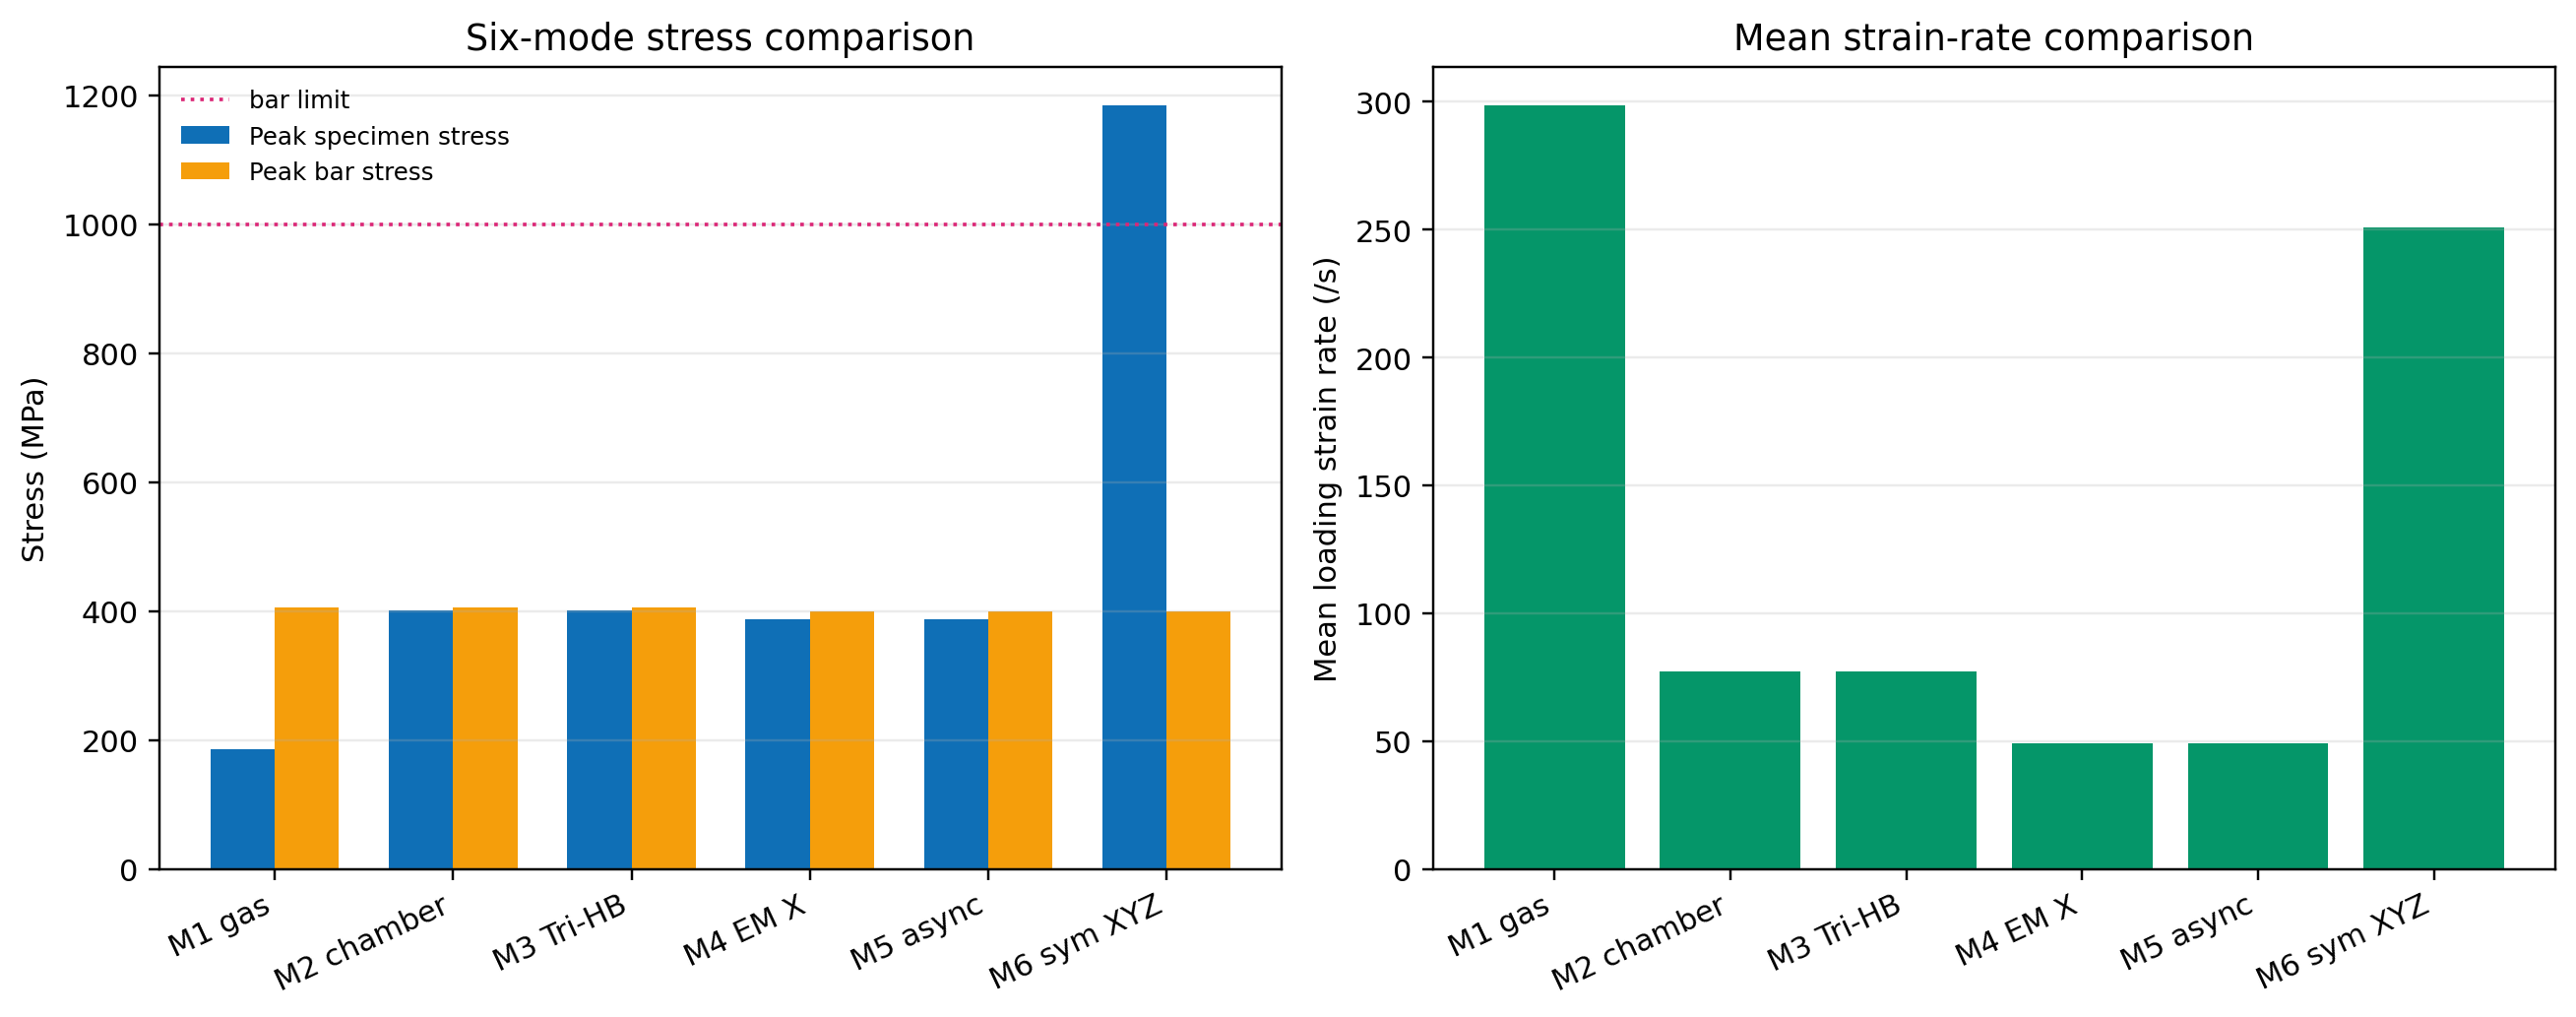
\includegraphics[width=\textwidth,height=0.74\textheight,keepaspectratio]{figures/handbook_modes/mode_comparison_summary.png}
  \end{figure}
\end{frame}

\begin{frame}{Mode 1: gas-gun uniaxial SHPB}
  \begin{columns}[T,onlytextwidth]
    \begin{column}{0.45\textwidth}
      \textbf{Use when:}
      \begin{itemize}
        \item Baseline dynamic uniaxial strength is the target.
        \item Published classical SHPB comparison is needed.
        \item Confinement and Lode-angle effects are outside scope.
      \end{itemize}
      \begin{block}{Main limitation}
        Single loading axis, no active confinement.
      \end{block}
    \end{column}
    \begin{column}{0.52\textwidth}
      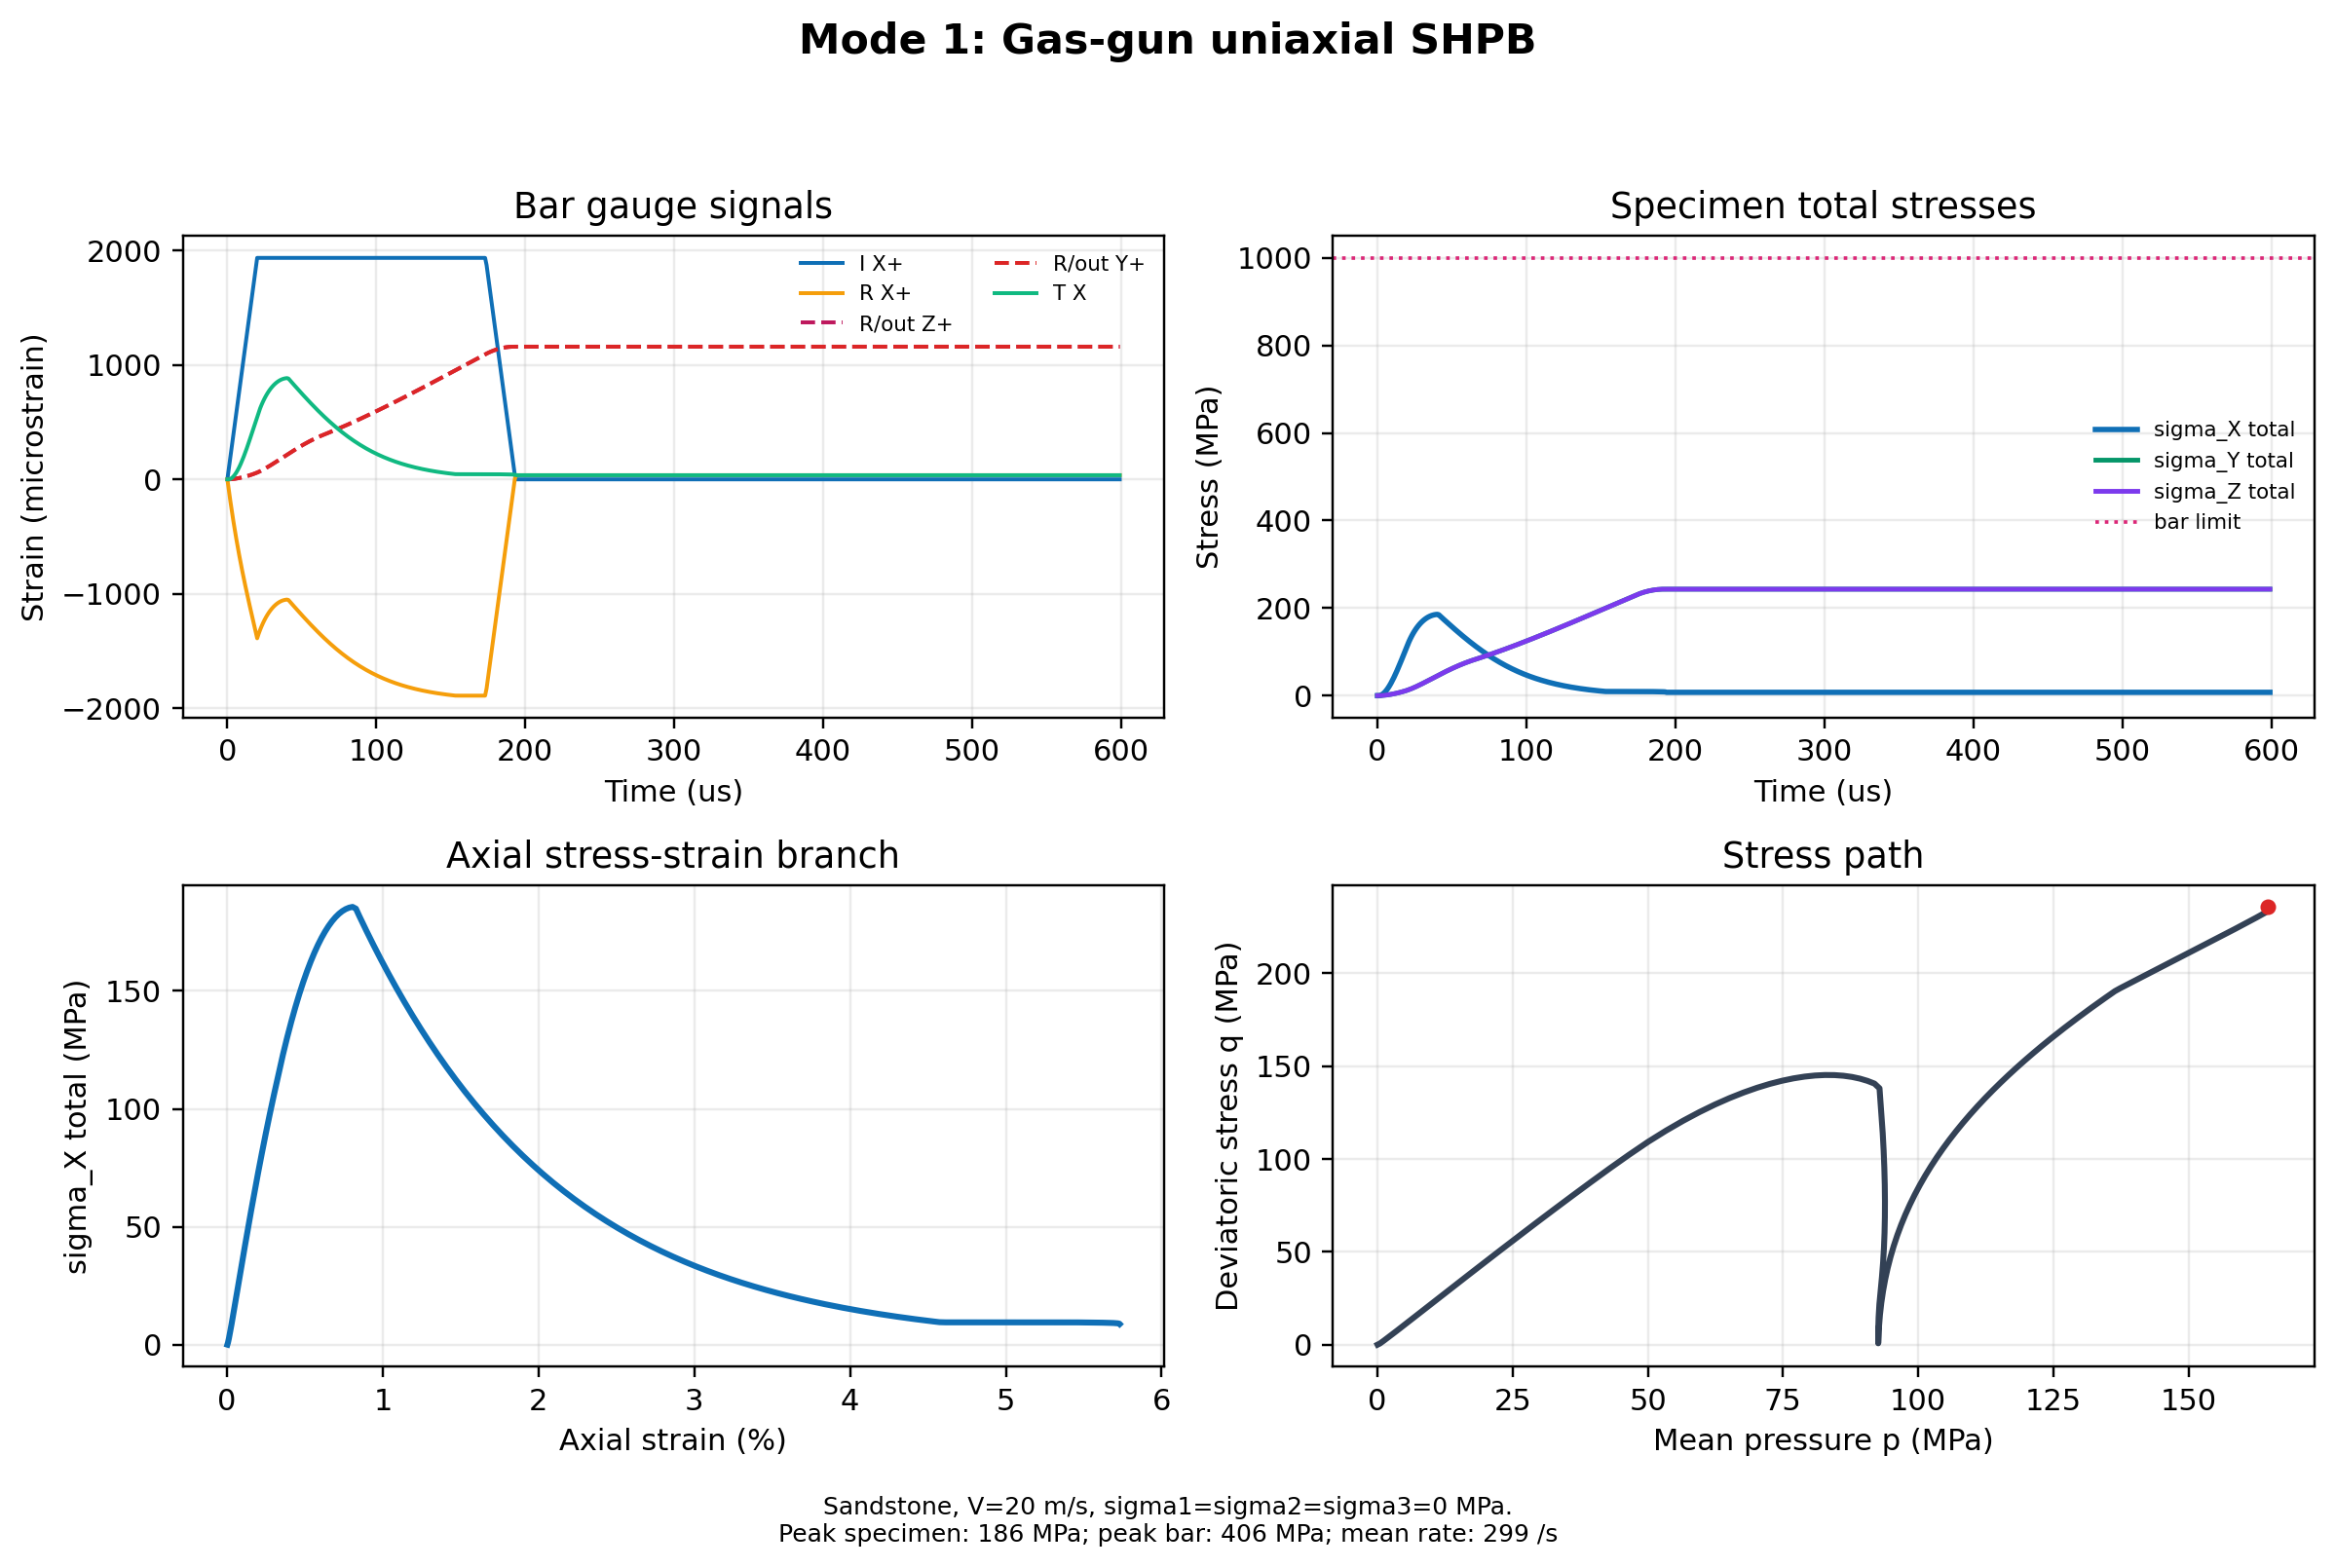
\includegraphics[width=\textwidth,height=0.66\textheight,keepaspectratio]{figures/handbook_modes/mode_1_gas_gun_uniaxial.png}
    \end{column}
  \end{columns}
\end{frame}

\begin{frame}{Mode 2: confinement-chamber SHPB}
  \begin{columns}[T,onlytextwidth]
    \begin{column}{0.45\textwidth}
      \textbf{Use when:}
      \begin{itemize}
        \item Axisymmetric triaxial confinement is sufficient.
        \item The specimen is cylindrical or jacketed.
        \item The stress path can remain at $\theta=0$.
      \end{itemize}
      \begin{block}{Main limitation}
        Lateral pressure is passive; independent $\sigma_2$ and $\sigma_3$
        cannot be imposed.
      \end{block}
    \end{column}
    \begin{column}{0.52\textwidth}
      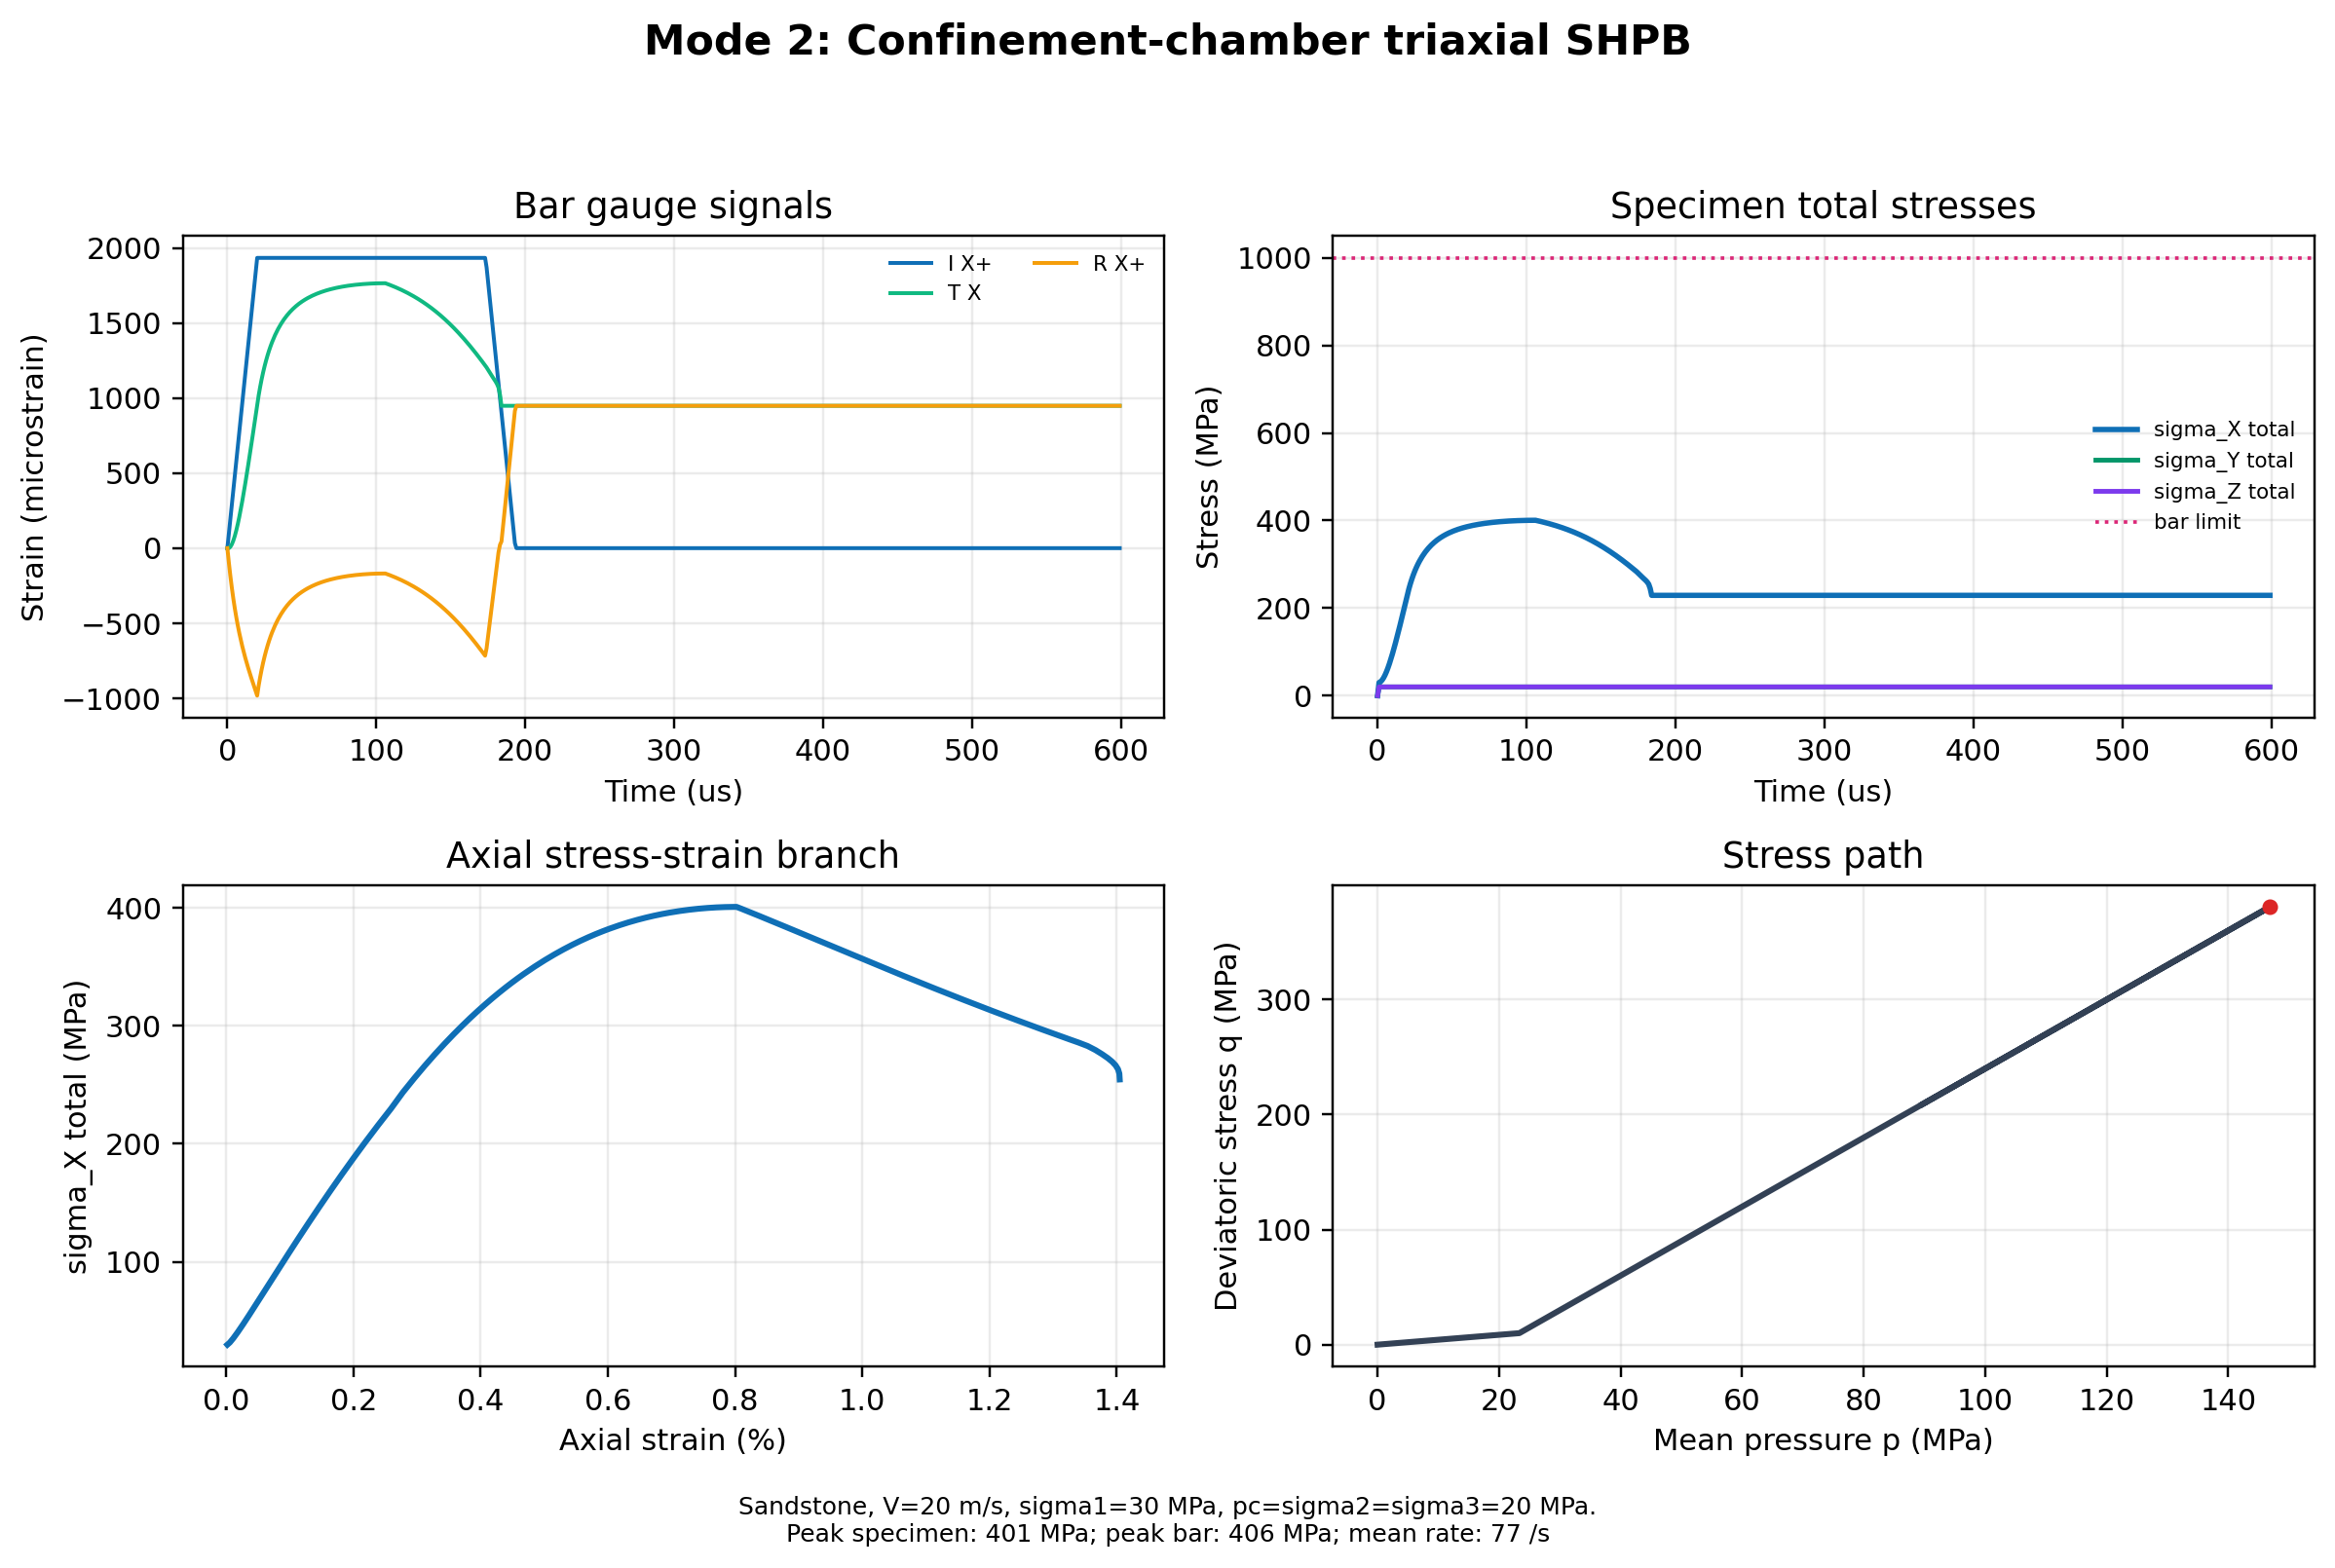
\includegraphics[width=\textwidth,height=0.66\textheight,keepaspectratio]{figures/handbook_modes/mode_2_confinement_chamber.png}
    \end{column}
  \end{columns}
\end{frame}

\begin{frame}{Mode 3: Monash gas-gun true triaxial loading}
  \begin{columns}[T,onlytextwidth]
    \begin{column}{0.45\textwidth}
      \textbf{Use when:}
      \begin{itemize}
        \item In-situ pre-stress matters.
        \item $\sigma_2$ and $\sigma_3$ must be independently controlled.
        \item Dynamic X loading is combined with true triaxial confinement.
      \end{itemize}
      \begin{exampleblock}{Signature capability}
        Gas-gun dynamic loading plus active orthogonal bar/cylinder confinement.
      \end{exampleblock}
    \end{column}
    \begin{column}{0.52\textwidth}
      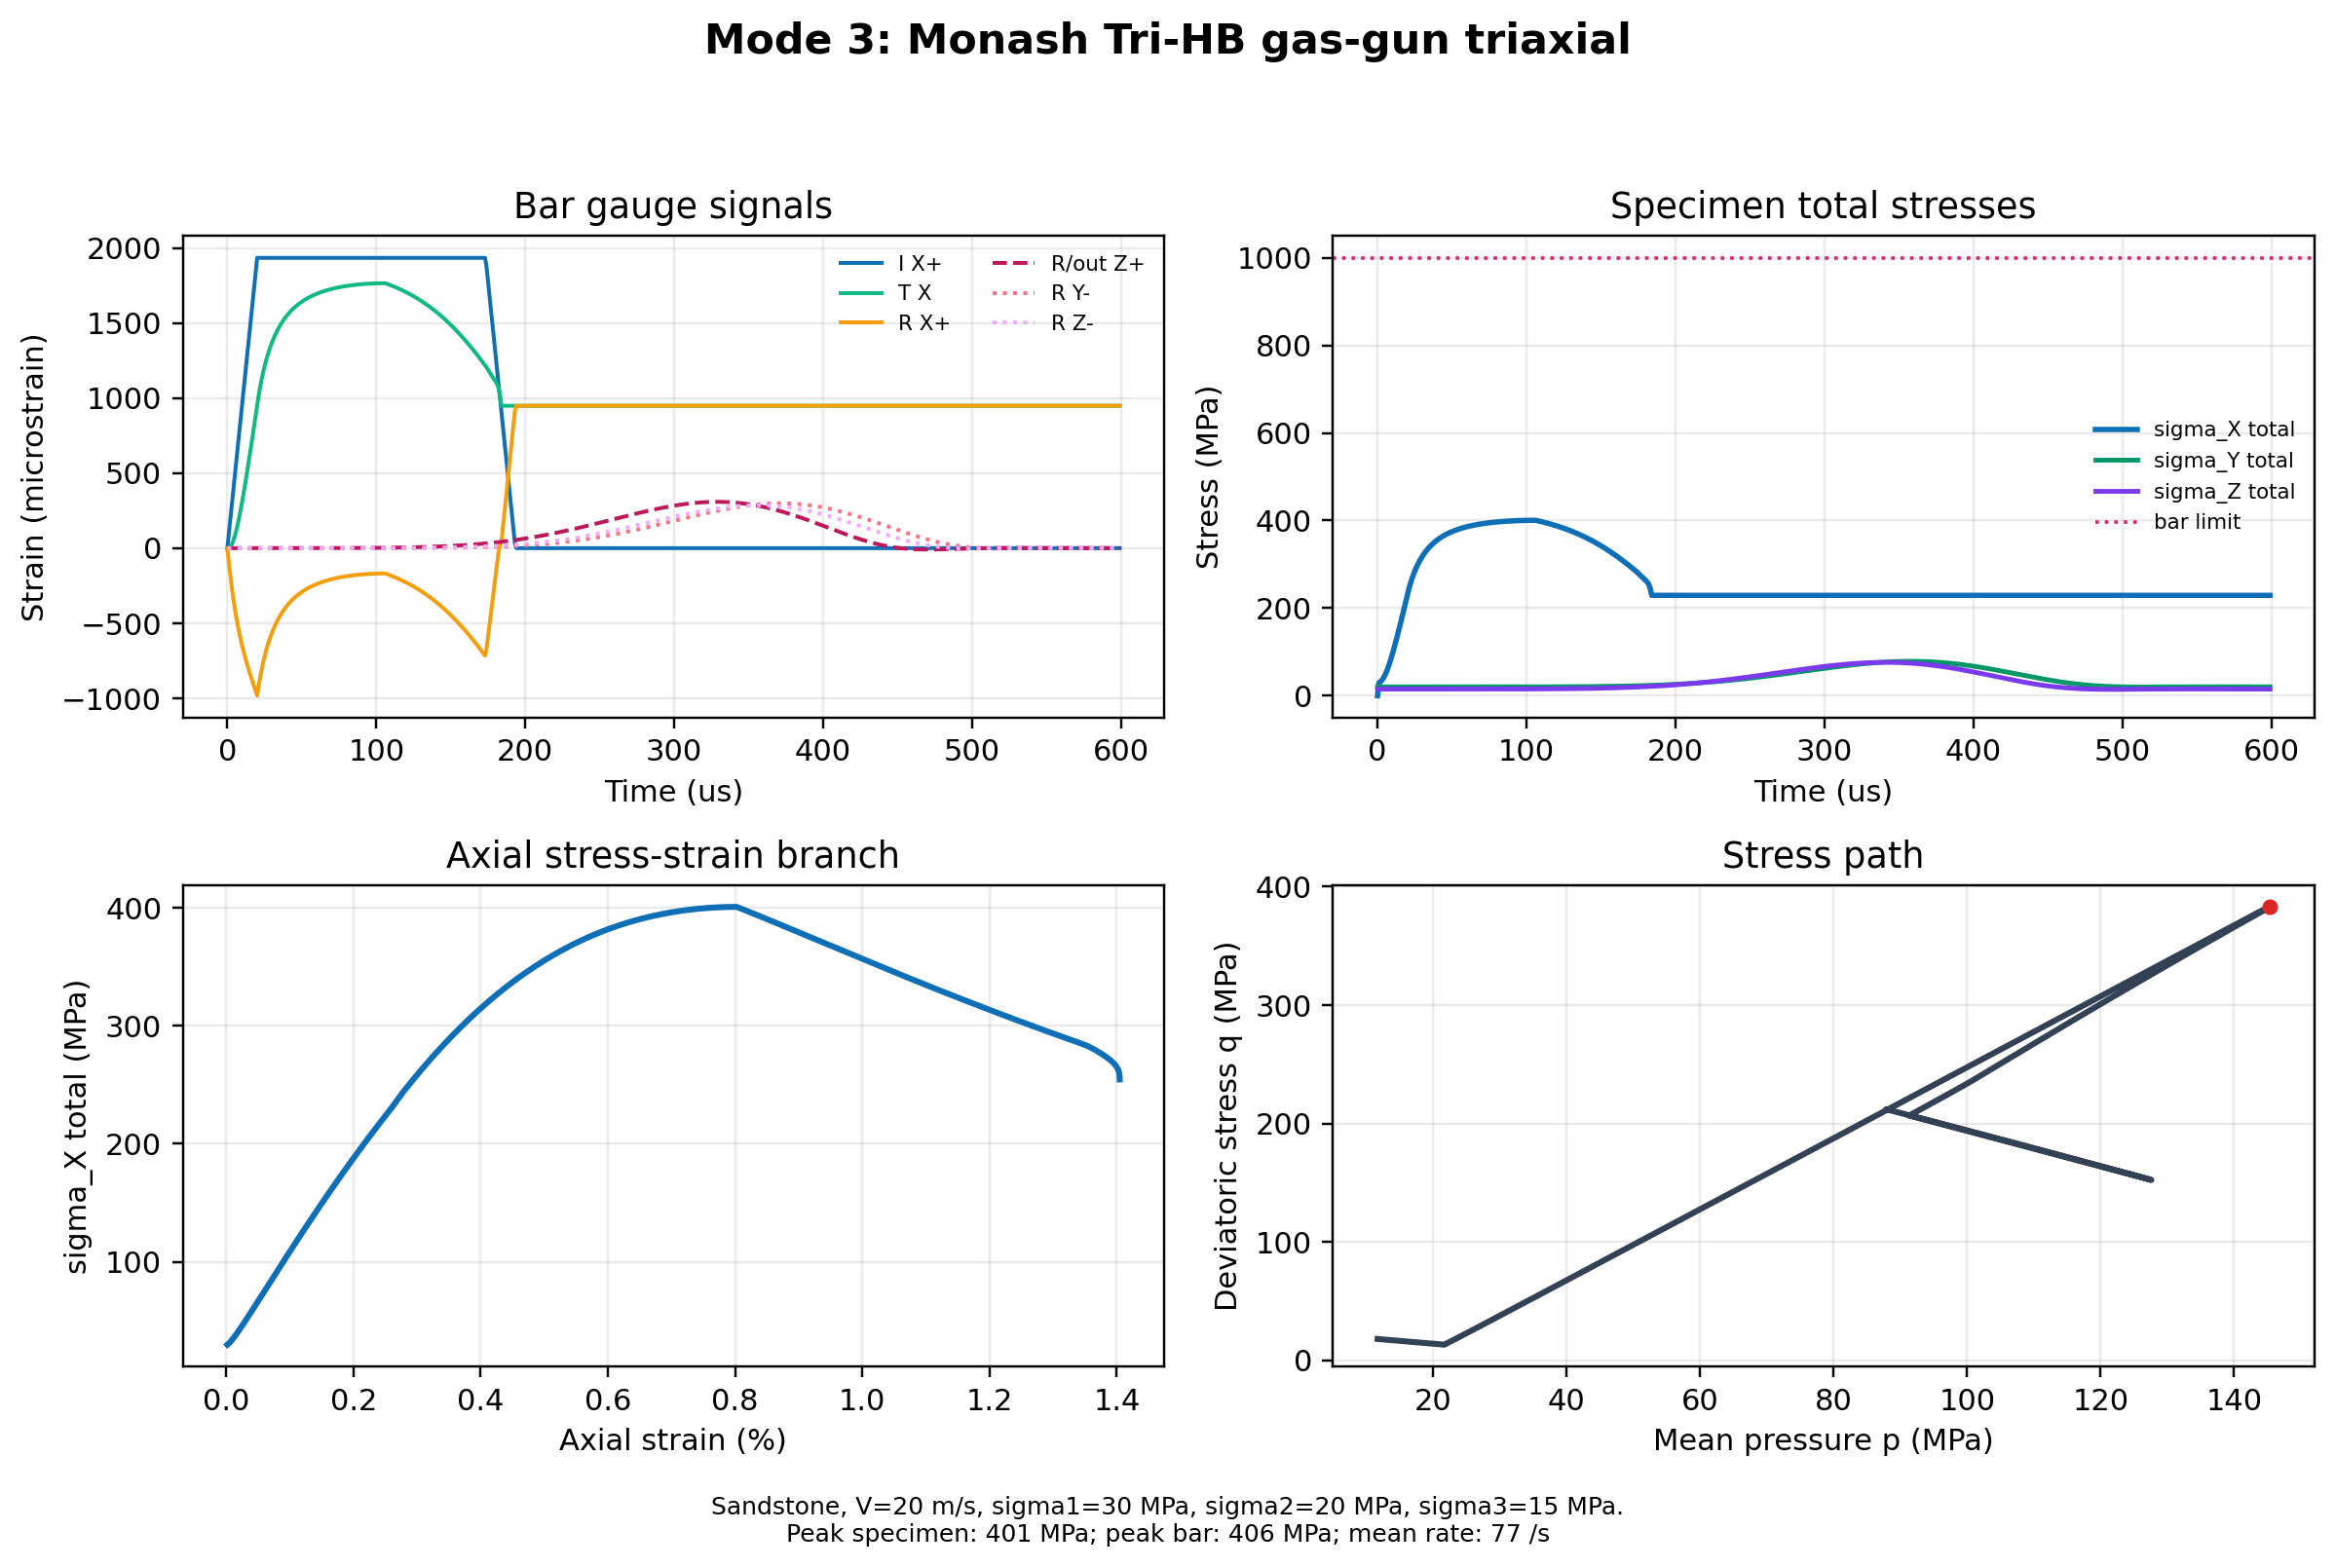
\includegraphics[width=\textwidth,height=0.66\textheight,keepaspectratio]{figures/handbook_modes/mode_3_monash_tri_hb.png}
    \end{column}
  \end{columns}
\end{frame}

\begin{frame}{Mode 4: electromagnetic uniaxial impact}
  \begin{columns}[T,onlytextwidth]
    \begin{column}{0.45\textwidth}
      \textbf{Use when:}
      \begin{itemize}
        \item A clean half-sine pulse is preferred.
        \item Pulse amplitude and duration must be tuned independently.
        \item Rate effects are the main research question.
      \end{itemize}
      \begin{block}{Design advantage}
        The EM system decouples peak stress from pulse duration.
      \end{block}
    \end{column}
    \begin{column}{0.52\textwidth}
      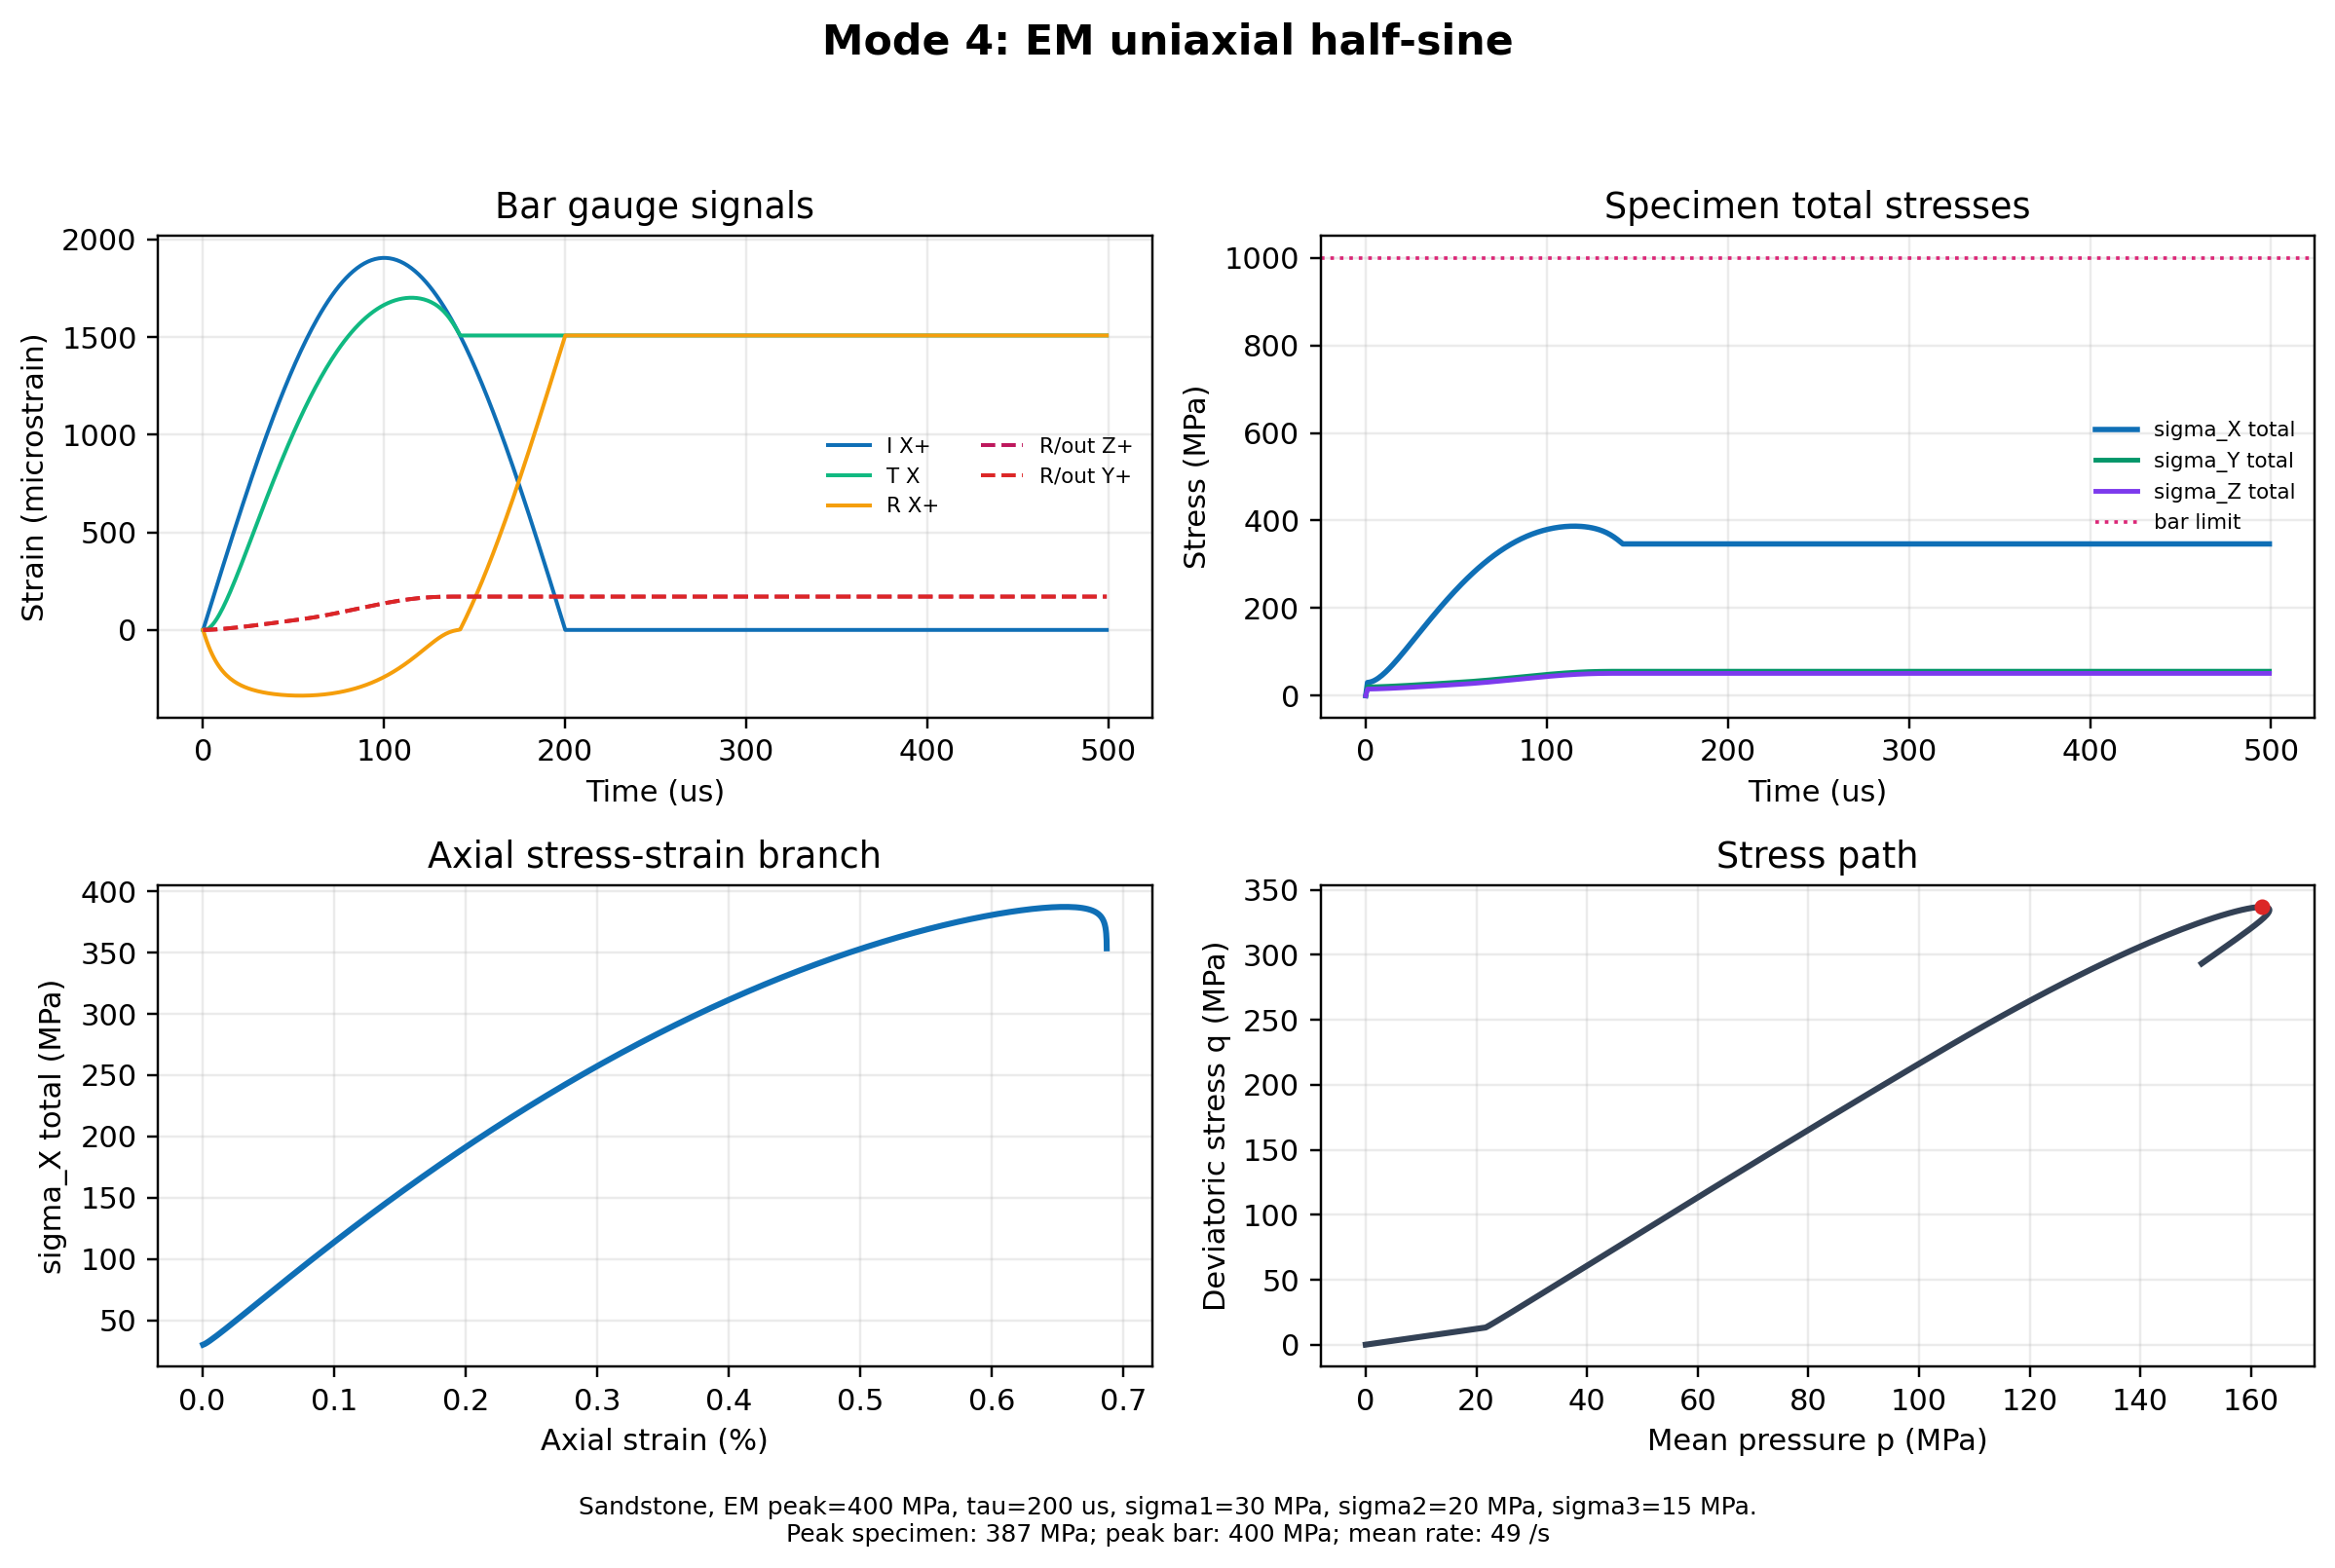
\includegraphics[width=\textwidth,height=0.66\textheight,keepaspectratio]{figures/handbook_modes/mode_4_em_uniaxial.png}
    \end{column}
  \end{columns}
\end{frame}

\begin{frame}{Mode 5: electromagnetic asynchronous triaxial impact}
  \begin{columns}[T,onlytextwidth]
    \begin{column}{0.45\textwidth}
      \textbf{Use when:}
      \begin{itemize}
        \item Loading order and inter-axis delay are the physics.
        \item Crack initiation may depend on which axis arrives first.
        \item Step 2 delay regime and Step 3 stress path are central outputs.
      \end{itemize}
      \begin{alertblock}{Interpretation warning}
        A uniaxial constitutive fit is not meaningful for asynchronous triaxial
        paths.
      \end{alertblock}
    \end{column}
    \begin{column}{0.52\textwidth}
      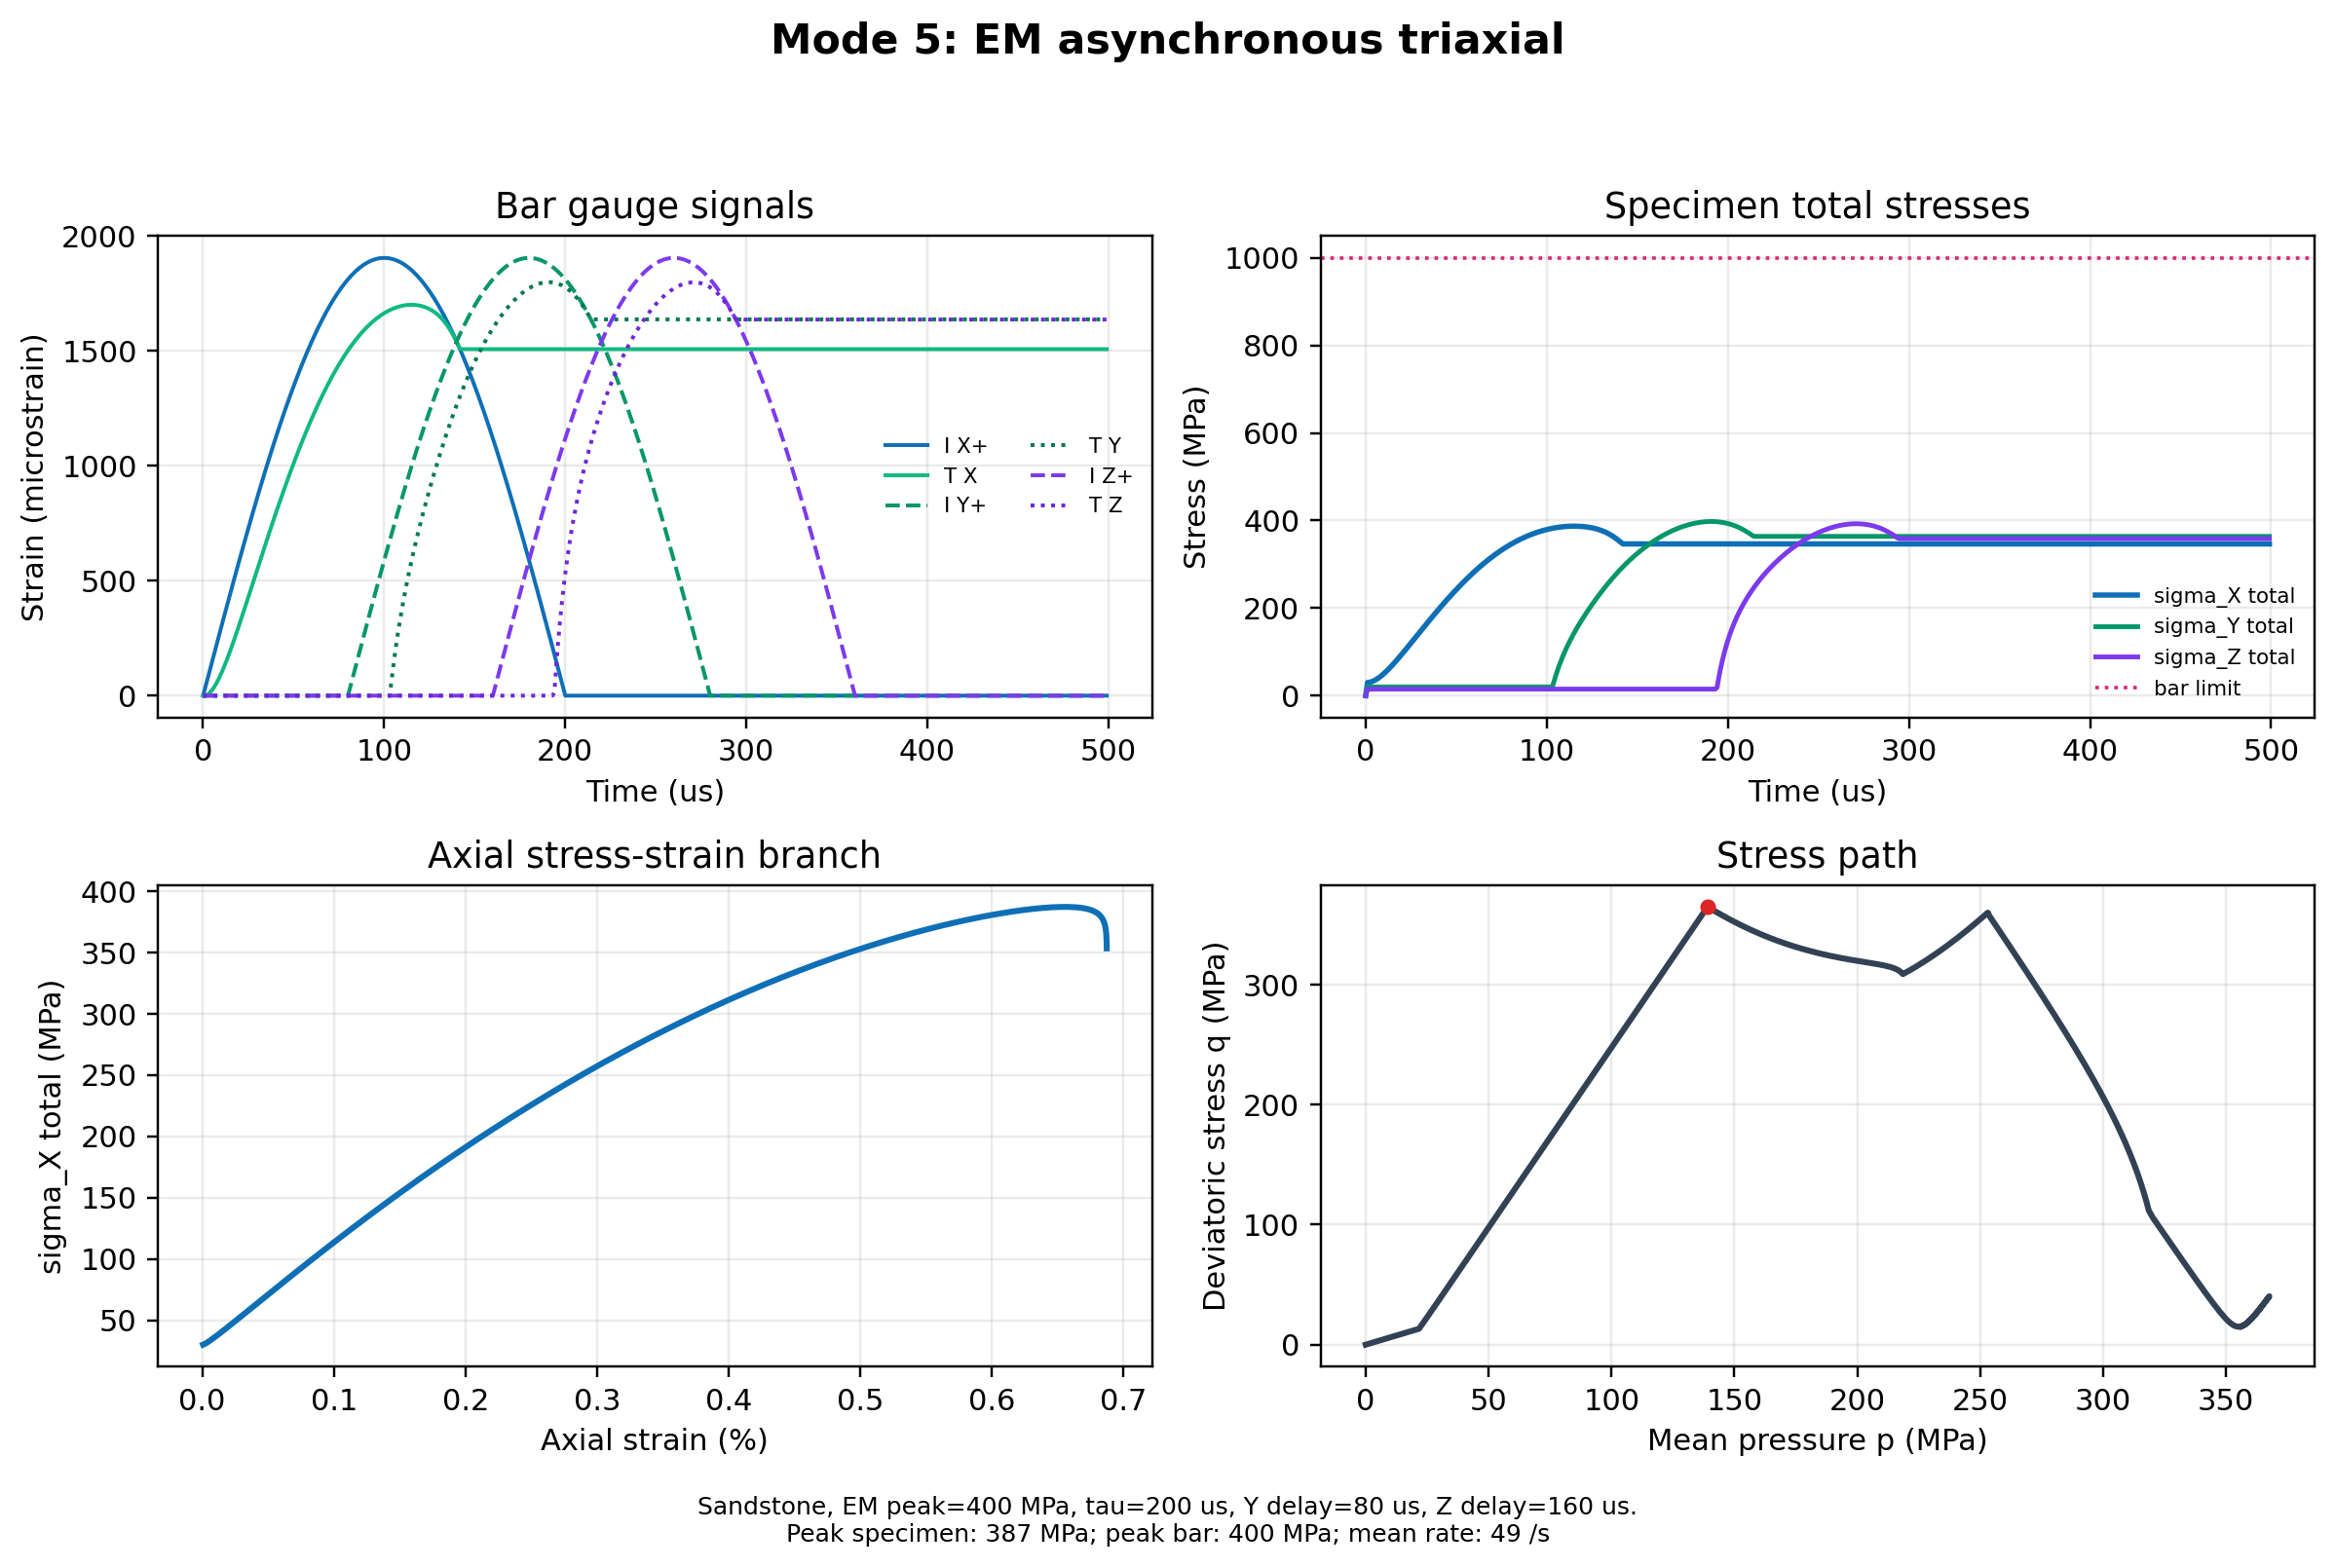
\includegraphics[width=\textwidth,height=0.66\textheight,keepaspectratio]{figures/handbook_modes/mode_5_em_async_triaxial.png}
    \end{column}
  \end{columns}
\end{frame}

\begin{frame}{Mode 6: electromagnetic symmetric multidirectional impact}
  \begin{columns}[T,onlytextwidth]
    \begin{column}{0.45\textwidth}
      \textbf{Use when:}
      \begin{itemize}
        \item Hydrostatic or near-hydrostatic dynamic loading is required.
        \item Specimen stress must exceed one-sided bar limits.
        \item Momentum cancellation is part of the design requirement.
      \end{itemize}
      \begin{exampleblock}{Key idea}
        Opposing pulses double specimen stress while keeping single-bar stress
        unchanged.
      \end{exampleblock}
    \end{column}
    \begin{column}{0.52\textwidth}
      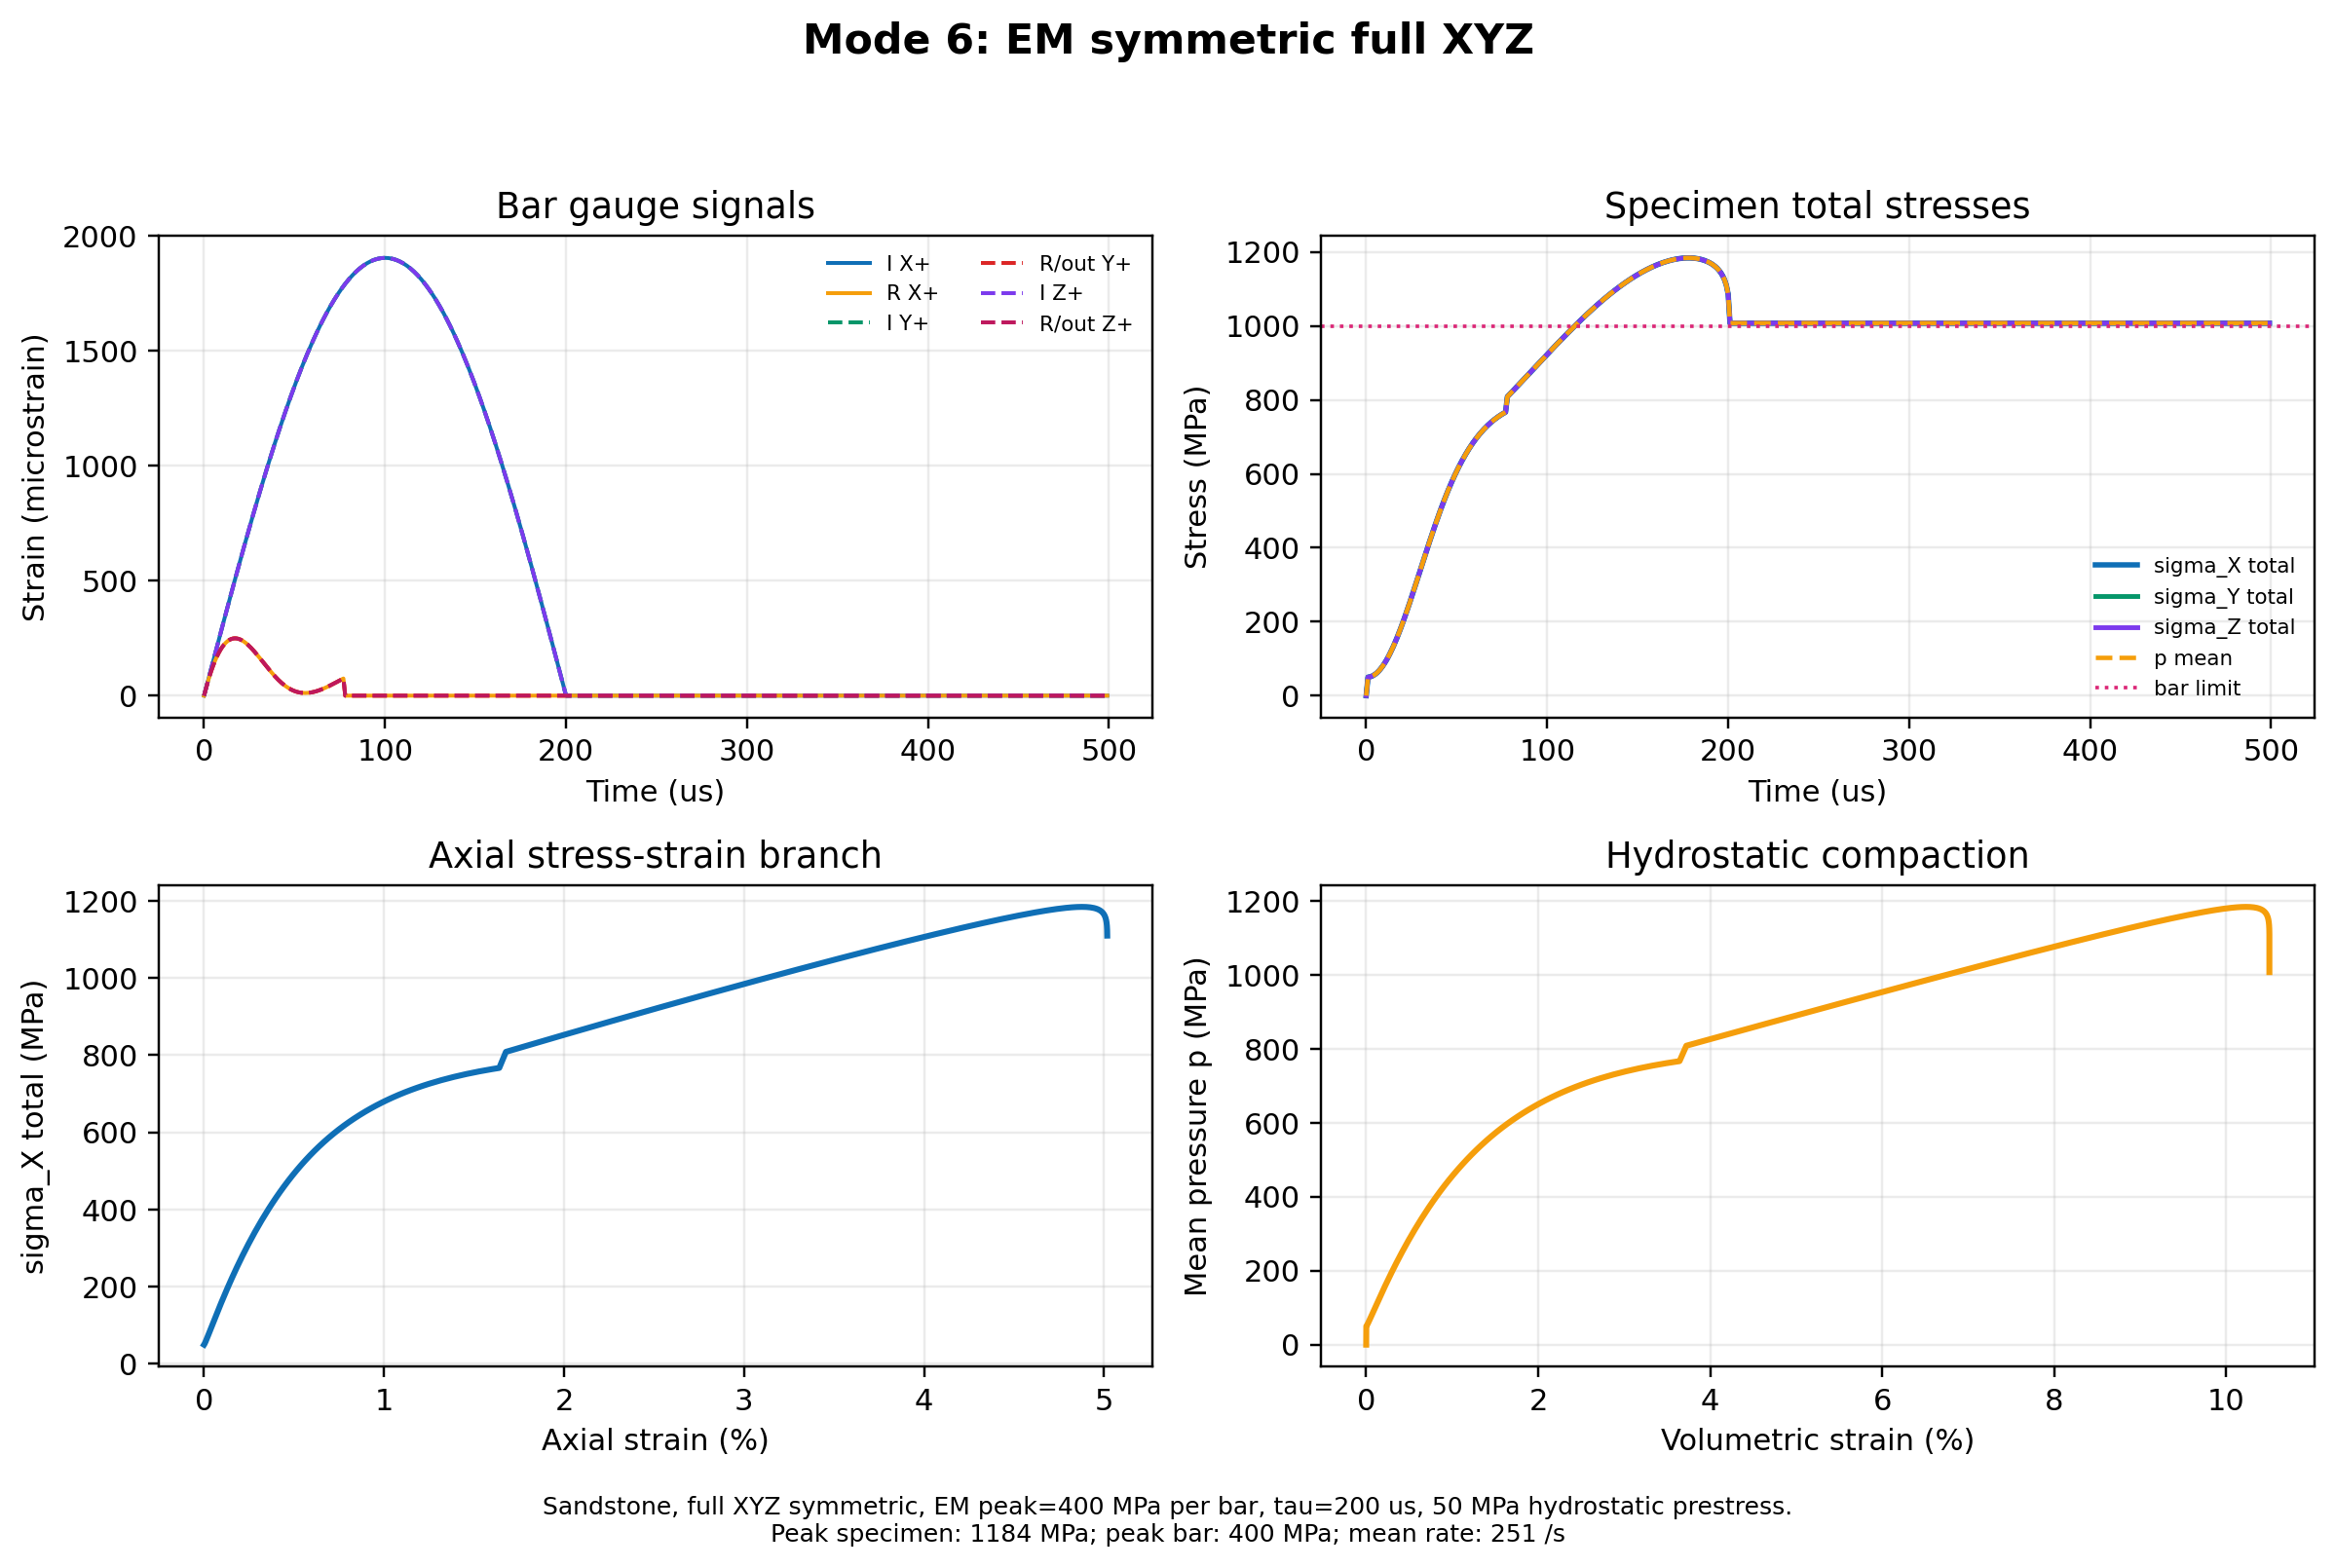
\includegraphics[width=\textwidth,height=0.66\textheight,keepaspectratio]{figures/handbook_modes/mode_6_em_symmetric_xyz.png}
    \end{column}
  \end{columns}
\end{frame}

\begin{frame}{Mode selection: match the apparatus to the question}
  \small
  \begin{tabular}{@{}p{0.18\textwidth}p{0.36\textwidth}p{0.36\textwidth}@{}}
    \toprule
    \textbf{Mode} & \textbf{Best question} & \textbf{Primary diagnostic} \\
    \midrule
    1 & Baseline dynamic strength & Three-wave equilibrium \\
    2 & Axisymmetric confinement & Confinement correction and $\theta=0$ \\
    3 & In-situ true triaxial pre-stress & Independent $\sigma_1,\sigma_2,\sigma_3$ \\
    4 & Clean rate sweep & Half-sine amplitude-duration control \\
    5 & Loading-order effects & $\Delta t^\ast$, $p$--$q$--$\theta$ path \\
    6 & Hydrostatic cap response & Symmetric energy folding and momentum cancellation \\
    \bottomrule
  \end{tabular}
  \vspace{0.35cm}
  \begin{block}{Practical rule}
    Choose the simplest mode that still preserves the stress state and timing
    physics required by the research question.
  \end{block}
\end{frame}

% ###################################################################
\section{Integrated Streamlit Workflow}
% ###################################################################

\begin{frame}{The integrated app is the operational front door}
  \begin{columns}[T,onlytextwidth]
    \begin{column}{0.48\textwidth}
      \begin{block}{Recommended launch}
        \cmdline{py -3.13 -m pip install -r requirements.txt}\\[4pt]
        \cmdline{py -3.13 -m streamlit run}\\
        \cmdline{tri_hb_integrated.py --server.port 8501}
      \end{block}
      \cncue{On macOS/Linux, replace \texttt{py -3.13} with the local launcher,
      commonly \texttt{python} or \texttt{python3}.}
    \end{column}
    \begin{column}{0.48\textwidth}
      \begin{exampleblock}{Loaded modules}
        \begin{itemize}
          \item \cmdline{Tri-HB.py}: Step 1 setup, simulator, export.
          \item \cmdline{wave_damage.py}: Steps 2--4 wave, stress path, damage,
                energy, validation.
        \end{itemize}
      \end{exampleblock}
    \end{column}
  \end{columns}
\end{frame}

\begin{frame}{Step 1 creates the shared experimental state}
  \begin{columns}[T,onlytextwidth]
    \begin{column}{0.48\textwidth}
      \textbf{Inputs}
      \begin{itemize}
        \item material preset and specimen geometry
        \item bar cross-section and elastic properties
        \item loading mode, pulse source, and pre-stress
        \item simulator or uploaded gauge data
      \end{itemize}
    \end{column}
    \begin{column}{0.48\textwidth}
      \textbf{Session-state handoff}
      \begin{block}{Shared keys}
        \cmdline{tri_hb_latest_config}\\
        \cmdline{tri_hb_latest_result}
      \end{block}
      These keep later steps synchronised with the current setup.
    \end{column}
  \end{columns}
\end{frame}

\begin{frame}{Step 2: wave timing and delay regime}
  \begin{figure}
    \centering
    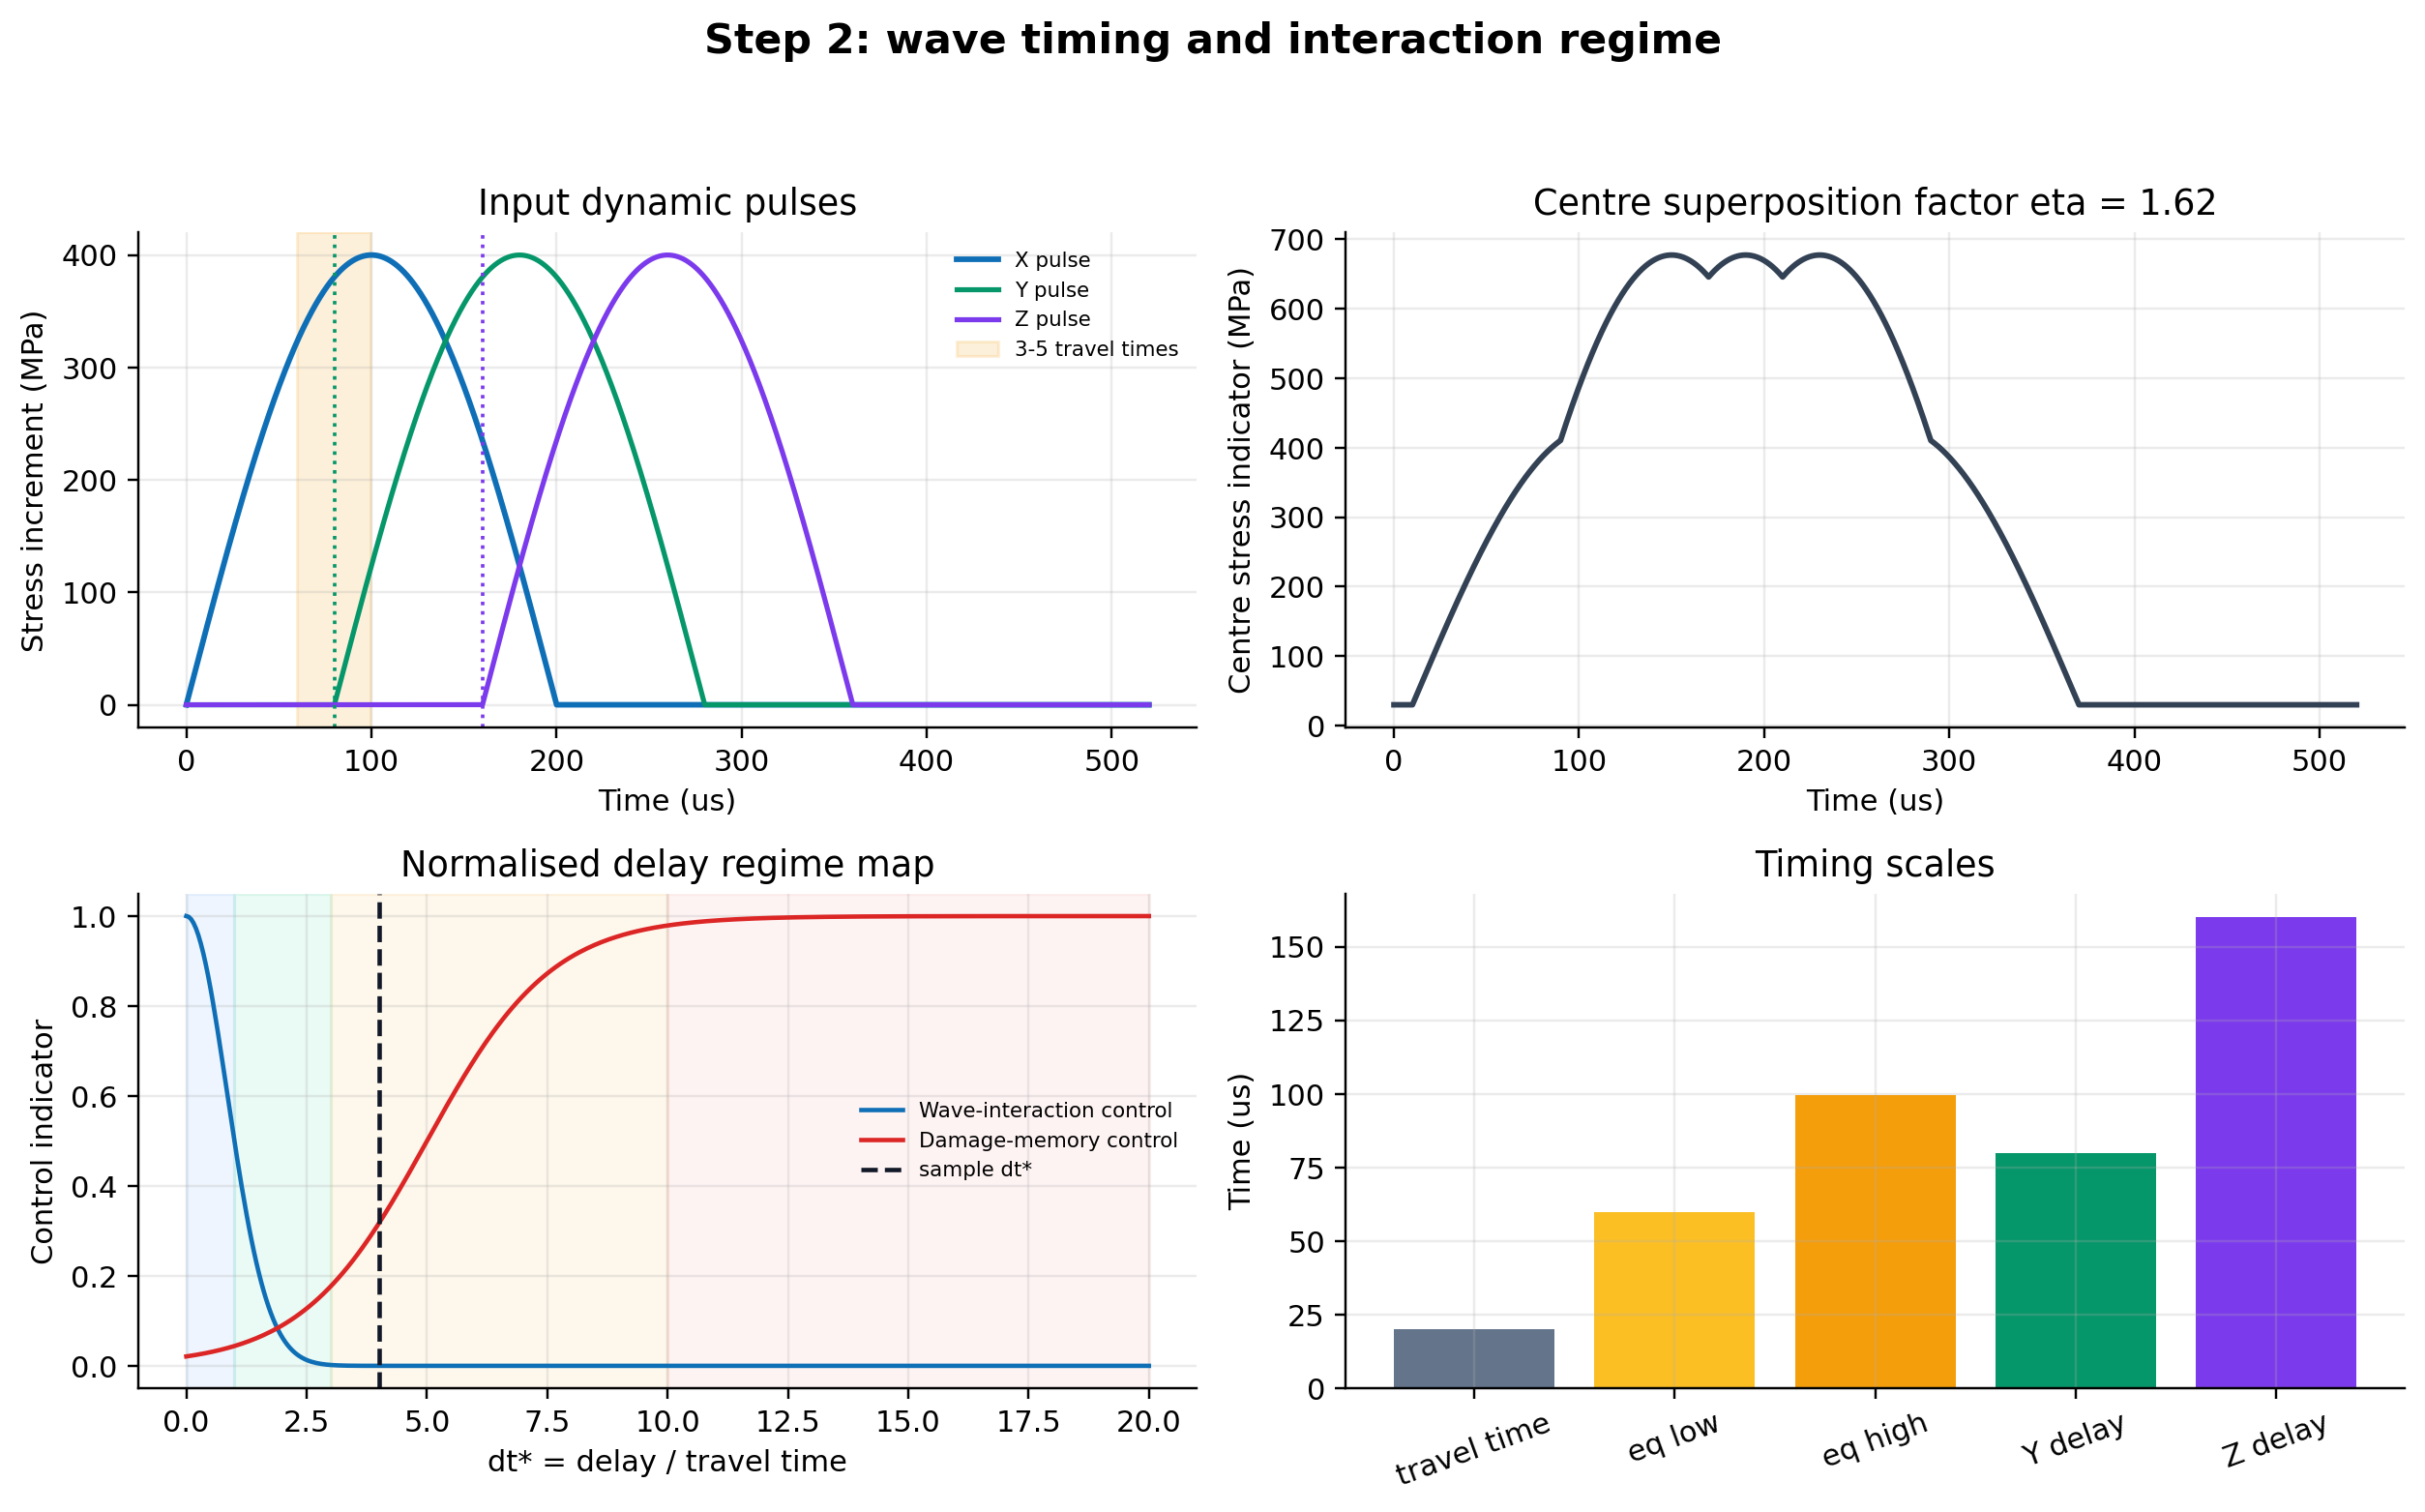
\includegraphics[width=\textwidth,height=0.75\textheight,keepaspectratio]{figures/handbook_steps/step2_wave_timing_regime.png}
  \end{figure}
\end{frame}

\begin{frame}{Step 3: stress path and failure index}
  \begin{figure}
    \centering
    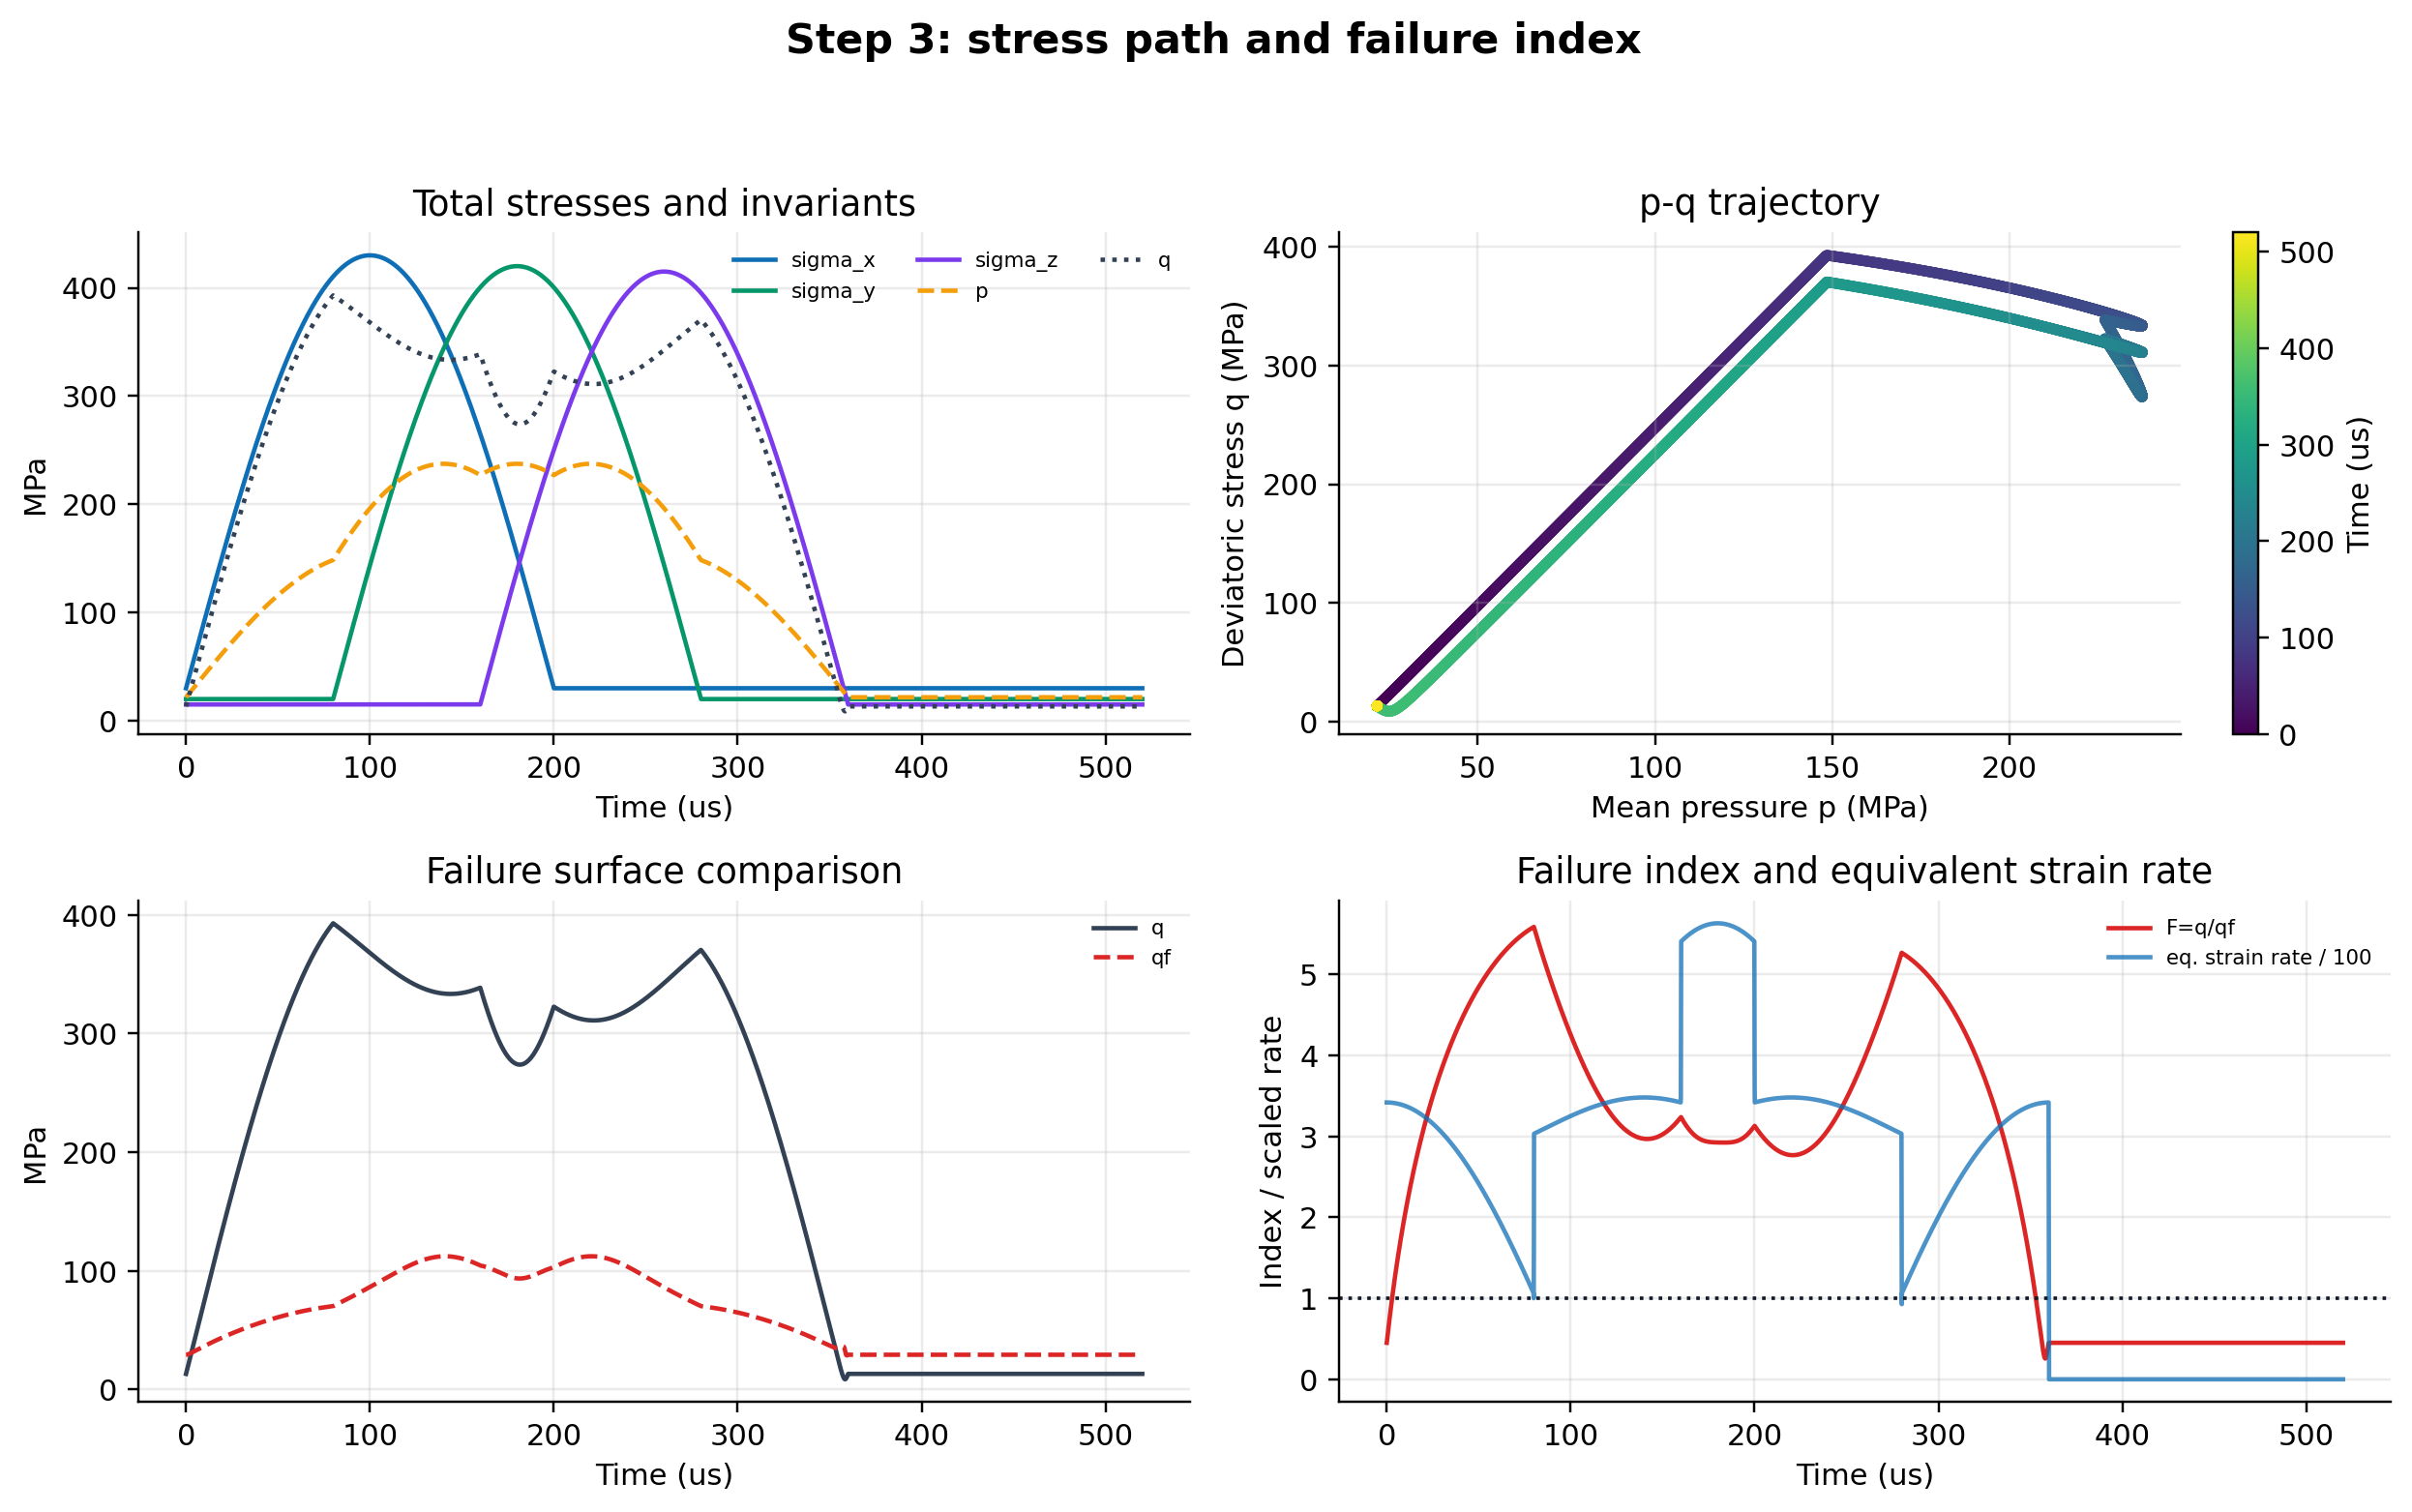
\includegraphics[width=\textwidth,height=0.75\textheight,keepaspectratio]{figures/handbook_steps/step3_stress_path_failure.png}
  \end{figure}
\end{frame}

\begin{frame}{Step 4: damage evolution and stiffness loss}
  \begin{figure}
    \centering
    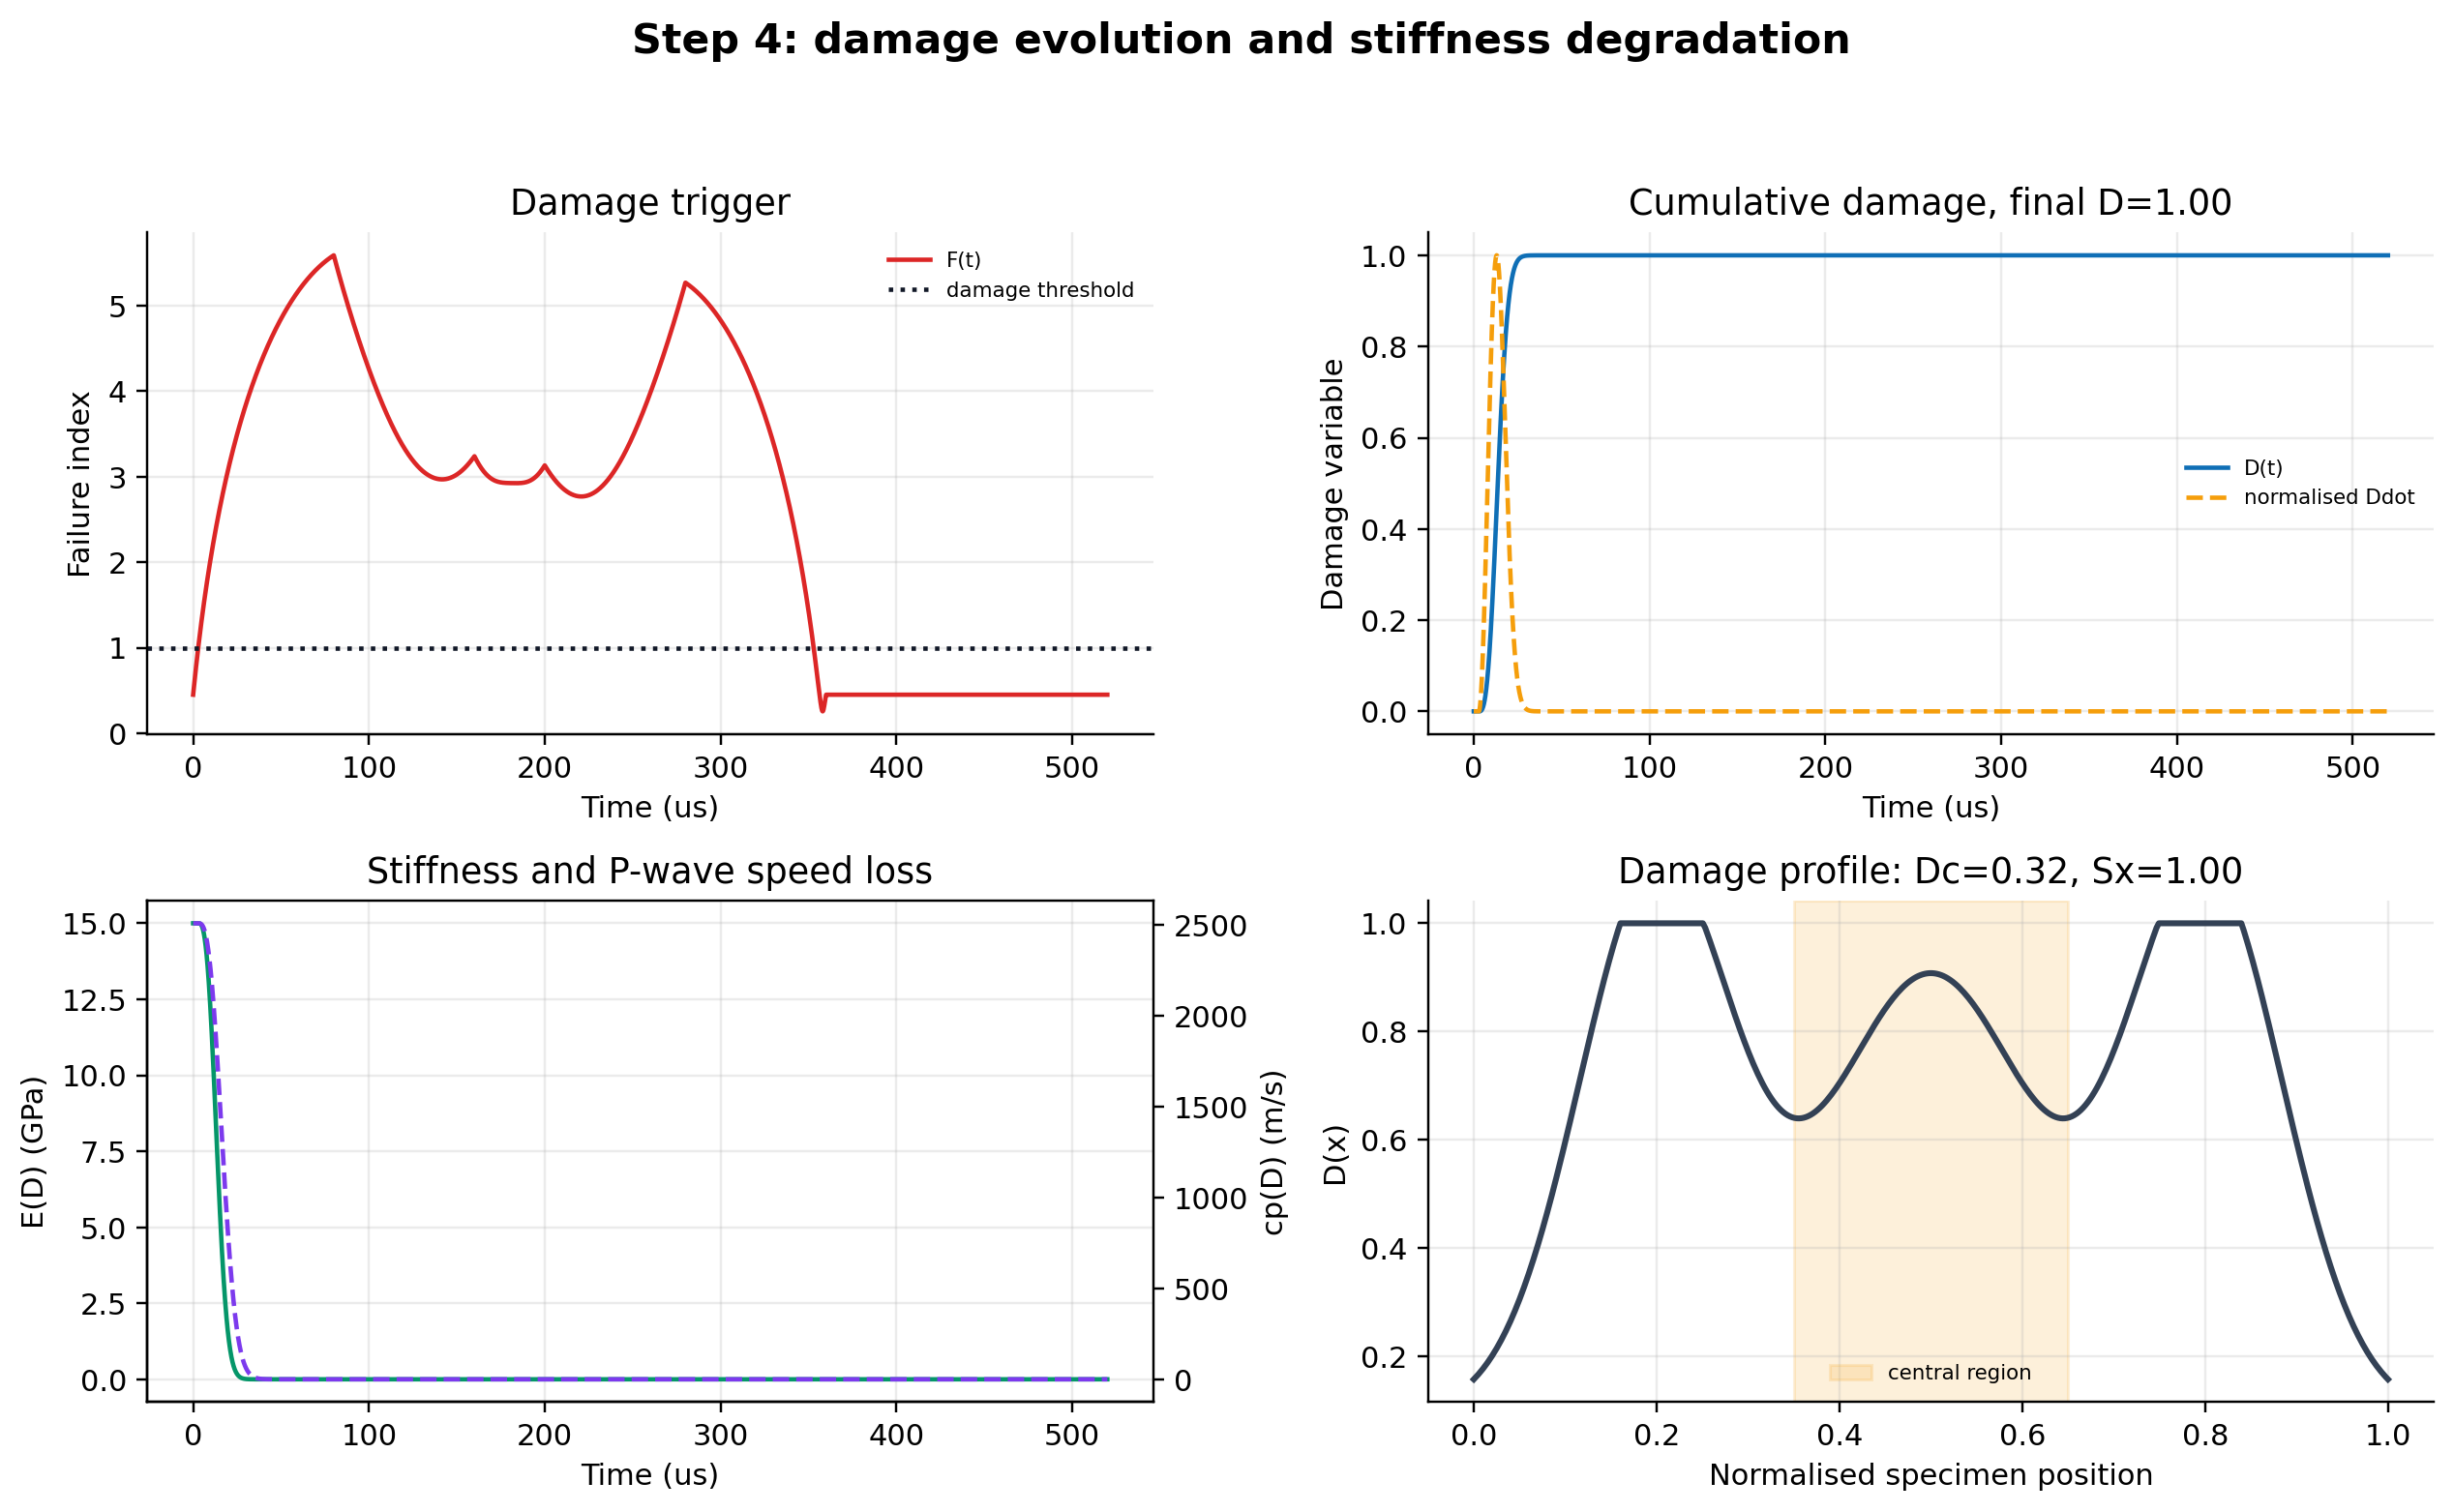
\includegraphics[width=\textwidth,height=0.75\textheight,keepaspectratio]{figures/handbook_steps/step4_damage_evolution.png}
  \end{figure}
\end{frame}

\begin{frame}{Step 4: energy density and validation descriptors}
  \begin{figure}
    \centering
    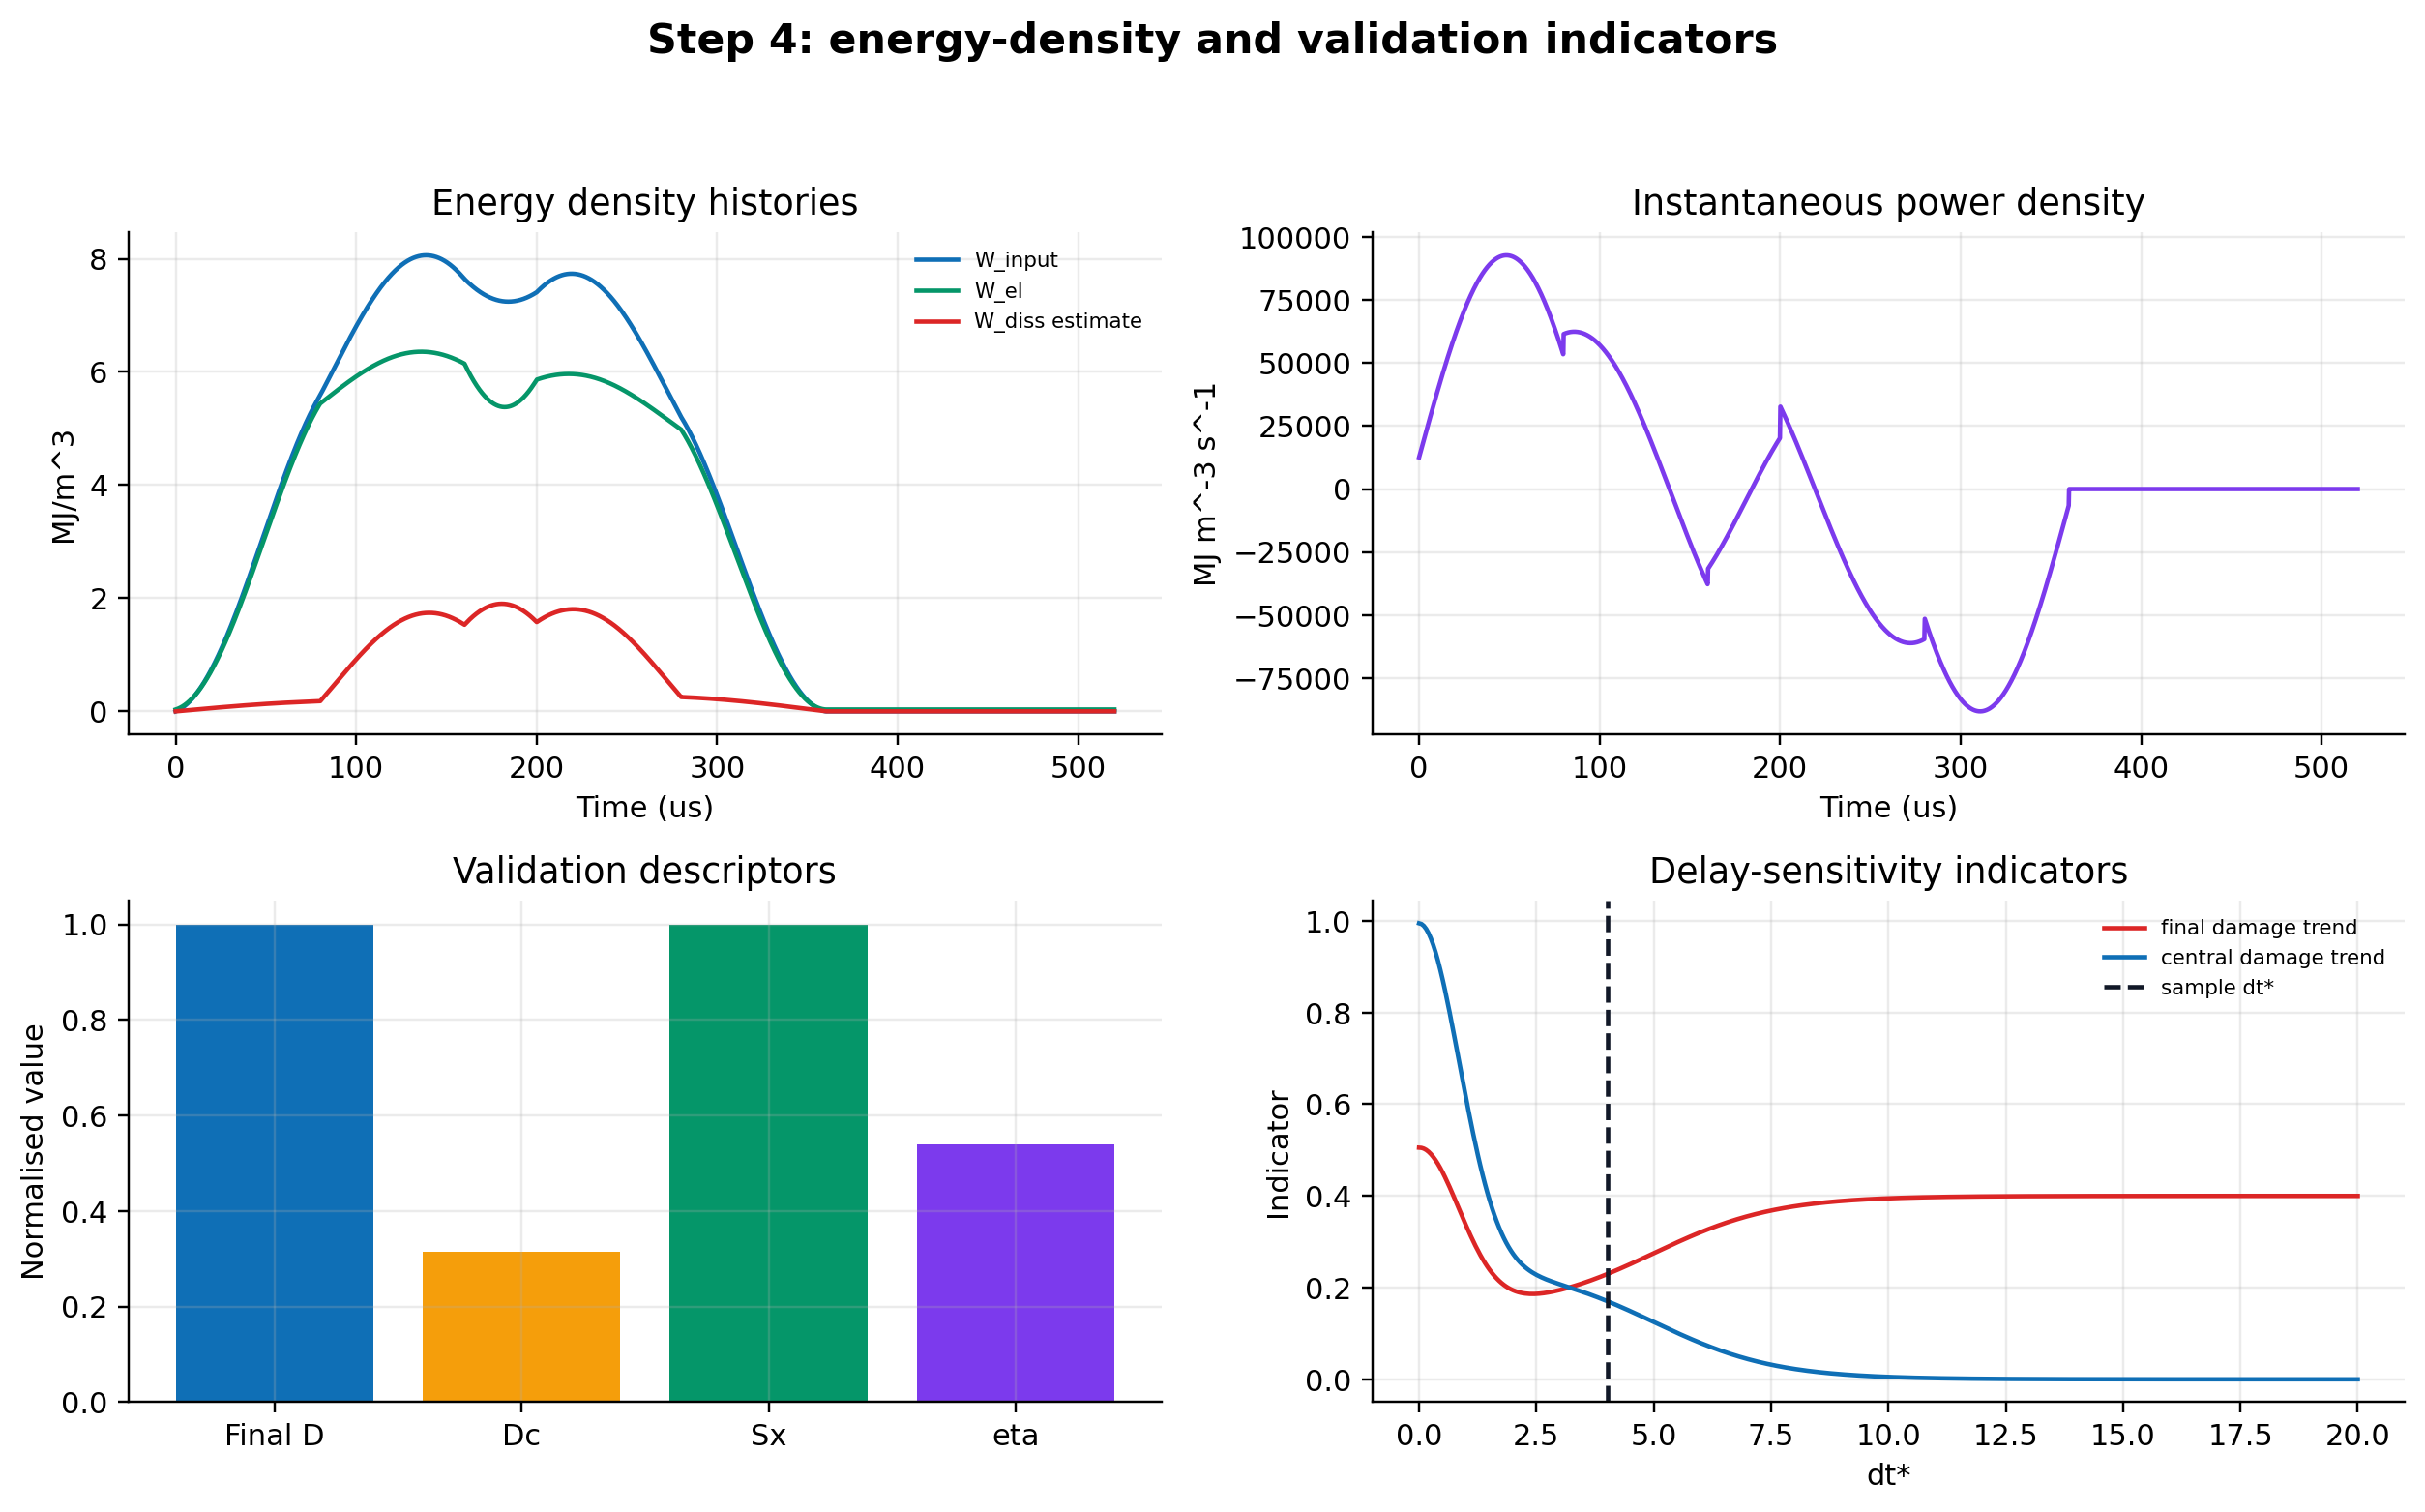
\includegraphics[width=\textwidth,height=0.75\textheight,keepaspectratio]{figures/handbook_steps/step4_energy_density_validation.png}
  \end{figure}
\end{frame}

\begin{frame}{Outputs connect the handbook to experiments}
  \begin{columns}[T,onlytextwidth]
    \begin{column}{0.48\textwidth}
      \begin{exampleblock}{Exportable data}
        \begin{itemize}
          \item stress--strain histories
          \item strain-rate histories
          \item incident/reflected/transmitted energies
          \item Step 2--4 CSV/XLSX summaries
        \end{itemize}
      \end{exampleblock}
    \end{column}
    \begin{column}{0.48\textwidth}
      \begin{block}{Validation targets}
        \begin{itemize}
          \item bar gauge amplitude and delay
          \item DIC localisation
          \item CT damage volume and crack orientation
          \item DEM bond breakage and dissipated energy
        \end{itemize}
      \end{block}
    \end{column}
  \end{columns}
\end{frame}

% ###################################################################
\section{Handbook V4 Deliverable}
% ###################################################################

\begin{frame}{What is new in this presentation-ready V4}
  \begin{itemize}
    \item Simulator presets and handbook equations are aligned around
          $\dot{\varepsilon}_{\mathrm{ref}}=10^{-5}\ \mathrm{s}^{-1}$.
    \item Six-mode figures are inserted into the corresponding apparatus
          chapters.
    \item Step 2--4 figures now document wave timing, stress path, damage,
          energy density, and validation descriptors.
    \item The launch instructions use the tested Windows launcher:
          \cmdline{py -3.13 -m streamlit}.
    \item Long inline code keys were reformatted to avoid PDF margin overflow.
  \end{itemize}
\end{frame}

\begin{frame}{Recommended use in teaching and research}
  \begin{columns}[T,onlytextwidth]
    \begin{column}{0.48\textwidth}
      \textbf{Teaching sequence}
      \begin{enumerate}
        \item start with Mode 1 wave reduction
        \item add confinement through Modes 2--3
        \item move to EM pulse control in Modes 4--6
        \item finish with Step 2--4 damage validation
      \end{enumerate}
    \end{column}
    \begin{column}{0.48\textwidth}
      \textbf{Research sequence}
      \begin{enumerate}
        \item choose mode from the stress-path question
        \item check bar plasticity and equilibrium
        \item export reduced histories
        \item calibrate damage and DEM descriptors
      \end{enumerate}
    \end{column}
  \end{columns}
\end{frame}

\begin{frame}{Closing}
  \begin{center}
    \Large Handbook V4 is now a linked system.\\[6pt]
    \normalsize Apparatus modes, equations, Streamlit workflow, figures, and
    validation outputs all point to the same calibration story.
  \end{center}
\end{frame}

\end{document}
